%%%%%%%%%%%%%%%%%%%%%%%%%%%%%%%%%%%%%%%%%%%%%%%%%%%%%%%%%%%%%%%%%%%%%%%%%%%%%%%%%%%%%%%%%%%%%%%%%%%%%%%%%%%%%%%
% Modèle de thèse LaTeX en français basé sur la classe book
% 
% Thomas Gaillard, juillet 2010, (CC) BY-SA.
% <thomas.gaillard@polytechnique.edu>
%
% Ce modèle est disponible sous licence Creative Commons paternité - partage à l¿identique.
% Une copie de cette licence est disponible à l'adresse <http://creativecommons.org/licenses/by-sa/3.0/deed.fr>
% ou par courrier à Creative Commons, 171 Second Street, Suite 300, San Francisco, California, 94105, USA.
%%%%%%%%%%%%%%%%%%%%%%%%%%%%%%%%%%%%%%%%%%%%%%%%%%%%%%%%%%%%%%%%%%%%%%%%%%%%%%%%%%%%%%%%%%%%%%%%%%%%%%%%%%%%%%%

\documentclass[a4paper,12pt]{book}
\usepackage[heightrounded,textheight=22.7658cm,vcentering,inner=3cm,outer=2cm]{geometry}
%\usepackage[heightrounded,top=3cm,bottom=3cm,inner=3cm,outer=2cm,verbose]{geometry}
\usepackage[utf8]{inputenc}   % le fichier .tex est en UTF-8
\usepackage[francais]{babel}  %typo française                    
\usepackage[T1]{fontenc}      % encodage des fonts latex         
\usepackage{lmodern}                                             
\usepackage{microtype}        % typo supplémentaires             

%%\usepackage[latin1]{inputenc}
%%\usepackage[T1]{fontenc}
%%\usepackage{lmodern}
%\usepackage[english,frenchb]{babel}

\usepackage{calc}
\usepackage{amsmath,amsfonts,amssymb}
\usepackage{graphicx}
\usepackage{color}
\usepackage{fancyhdr}
\usepackage{indentfirst}
\frenchspacing
\usepackage{setspace}
\onehalfspacing
\usepackage{float}
\usepackage[authoryear,square,colon]{natbib}
\bibpunct{[}{]}{\,;}{a}{}{,}
\bibliographystyle{bibliostyle}
\usepackage{array}
\usepackage{multirow}
\usepackage{multicol}
\usepackage{xspace}
\usepackage[plainpages=false,pdfpagelabels,pagebackref]{hyperref}
\pdfcompresslevel=9
\hypersetup{%
  pdftitle={Titre de la thèse}, 
  pdfauthor={David Mignon},
  pdfkeywords={motclé1,motclé2,motclé3},
  pdfsubject={Thèse de doctorat},
  colorlinks=true,
  linkcolor=black,
  urlcolor=black,
  citecolor=black
}

% Titlepage adjustment
\addtolength{\textheight}{+3cm}
\addtolength{\topmargin}{-1.5cm}
\addtolength{\oddsidemargin}{-0.5cm}
\addtolength{\evensidemargin}{+0.5cm}

% Pages où se trouvent les citations
\renewcommand*{\backref}[1]{}
\renewcommand*{\backrefalt}[4]{%
  % alternative interface
  % #1: number of distinct back references
  % #2: backref list with distinct entries
  % #3: number of back references including duplicates
  % #4: backref list including duplicates
  \par
  \nopagebreak
  \ifnum#1=1 %
    \ifnum#3=1 %
      {\small cité page~}%
    \else
      {\small cité page~}%
    \fi
  \else
    {\small cité pages~}%
  \fi
  {\small#2}\par
}
\renewcommand*{\backrefsep}{, }
\renewcommand*{\backreftwosep}{ et~}
\renewcommand*{\backreflastsep}{ et~}

% Pas d'espace après la virgule en mode mathématique
\DecimalMathComma

\makeatletter
% Custom titlepage
\def\maketitle{
\thispagestyle{empty}
\noindent
\begin{minipage}[b]{0.2\textwidth}
\begin{flushleft}
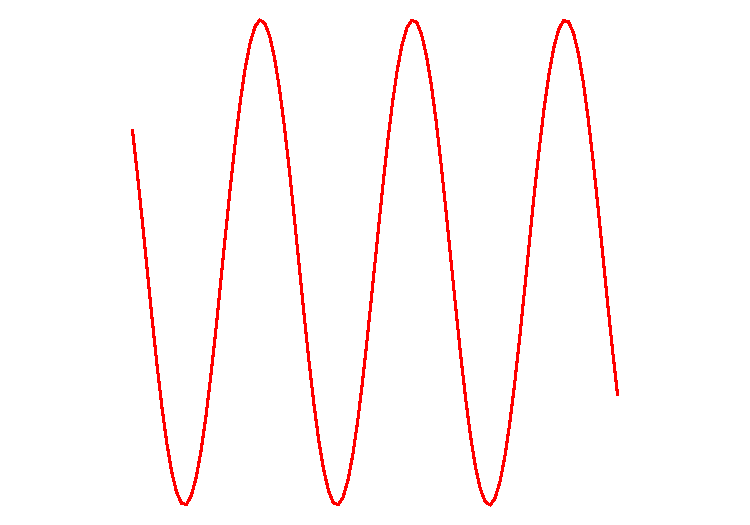
\includegraphics[width=0.85\textwidth]{logo.pdf}
\end{flushleft}
\end{minipage}
\hfill
\begin{minipage}[b]{0.75\textwidth}
{\footnotesize \bf \hfill Institut de XXX\\}
\vspace{-\baselineskip}
\vspace{2ex}
\hrule
\vspace{1.5ex}
{\footnotesize \bf \hfill École Doctorale de XXX}
% \end{minipage}
% \vfill
\begin{center}
{\LARGE \bf \@title\\}
\vfill
{\LARGE \bf THÈSE\\}
\vspace{4ex}
{\small présentée et soutenue publiquement le \@date\\}
\vspace{2ex}
{\small pour l'obtention du\\}
\vspace{4ex}
{\large \bf Doctorat de l'Université XXX\\}
\vspace{1ex}
{\small \bf (spécialité XXX)\\}
\vspace{2ex}
{\small par\\}
\vspace{1ex}
{\large \@author\\}
\end{center}
\vfill
\begin{small}
{\bf Composition du jury}
\begin{center}
\begin{tabular}{lll}
Rapporteurs :  & Dr. Prénom1 \bsc{Nom1} & Rapporteur externe\\
               & Dr. Prénom2 \bsc{Nom2} & Rapporteur externe\\
               & Pr. Prénom3 \bsc{Nom3} & Rapporteur interne\\
               & &\\
Examinateurs : & Dr. Prénom4 \bsc{Nom4} & Examinateur\\
               & Dr. Prénom5 \bsc{Nom5} & Directeur de thèse\\
               & Dr. Prénom6 \bsc{Nom6} & Directeur de thèse\\
\end{tabular}
\end{center}
\end{small}
\vfill
\begin{center}
\hrule
\vspace{2ex}
{\footnotesize \bf Laboratoire de XXX}
\end{center}
\newpage
\thispagestyle{empty}
\null
\addtolength{\textheight}{-3cm}
\addtolength{\topmargin}{+1.5cm}
\addtolength{\oddsidemargin}{+0.5cm}
\addtolength{\evensidemargin}{-0.5cm}
}
% Custom chapter % Careful : unnumbered chapters are not redefined in the same way
\def\@makechapterhead#1{%
\vspace*{50\p@}%
{\parindent \z@
\ifnum \c@secnumdepth >\m@ne
\colorbox{gray}{\parbox{\textwidth-\marginparsep}{\vspace{2pt}\Large\bfseries \@chapapp\space \thechapter}}
\par\nobreak
\fi
\interlinepenalty\@M
\raggedright \normalfont \Huge \bfseries #1
\par\nobreak
\vskip 40\p@
}}
%% Custom section
%\renewcommand\section{
%\@startsection{section}{1}{\z@}%
%{-3.5ex \@plus -1ex \@minus -.2ex}%
%{2.3ex \@plus.2ex}%
%{\color{gold}\reset@font\Large\sffamily\bfseries}}
%% Custom subsection
%\renewcommand\subsection{
%\@startsection{subsection}{2}{\z@}%
%{-3.25ex\@plus -1ex \@minus -.2ex}%
%{1.5ex \@plus .2ex}%
%{\reset@font\large\sffamily\bfseries}}
%% Custom subsubsection
%\renewcommand\subsubsection{
%\@startsection{subsubsection}{3}{\z@}%
%{-3.25ex\@plus -1ex \@minus -.2ex}%
%{1.5ex \@plus .2ex}%
%{\reset@font\normalsize\sffamily\bfseries}}
\makeatother

% Define colors
\definecolor{gold}{rgb}{0.75,0.5,0}
\definecolor{lightgold}{rgb}{1,.9,.4}
\definecolor{gray}{rgb}{.8,.8,.8}

% Negative space to remove automatic spacing
\newcommand\negspace{\hspace{-0.3em}}

% Pénalités pour les lignes isolées
\widowpenalty=10000
\clubpenalty=10000
\raggedbottom

% Placement des flottants
\renewcommand{\topfraction}{0.85} % 0.70
\renewcommand{\textfraction}{0.1} % 0.20
\renewcommand{\floatpagefraction}{0.75} % 0.50

% Noms des flottants et titres des listes
\addto\captionsfrench{%
   \def\figurename{Figure}%
   \def\tablename{Table}%
   \def\listfigurename{Liste des figures}%
   \def\listtablename{Liste des tables}%
}

% Gestion des en-têtes
\pagestyle{fancy}
\fancyhf{}
\fancyhead[LE]{\nouppercase{\bfseries\slshape\leftmark}}
\fancyhead[RO]{\nouppercase{\bfseries\slshape\rightmark}}
\fancyfoot[LE,RO]{\nouppercase{\bfseries\thepage}}
\addtolength{\headheight}{2.5pt} % espace pour le filet
\fancypagestyle{plain}{ % pages de têtes de chapitre
  \fancyhead{}         % supprime l'en-tête
  \renewcommand{\headrulewidth}{0pt} % et le filet
}

% Page sans en-têtes et pied de page
\newcommand{\clearemptydoublepage}{%
\newpage{\pagestyle{empty}\cleardoublepage}}

% Page sans en-têtes
\newcommand{\clearplaindoublepage}{%
\newpage{\pagestyle{plain}\cleardoublepage}}


\title{Titre de la thèse}

\author{David \bsc{Mignon}}

\date{XXX}

\begin{document}

% Title
\pagenumbering{alph}
\pdfbookmark[0]{Couverture}{cover}
\maketitle 
\clearemptydoublepage

% Frontmatter
\frontmatter
\thispagestyle{plain}
\pdfbookmark[0]{Remerciements}{acknowledgements}
\chapter*{Remerciements}

Je remercie les membres du jury, Julien Bigot, Alain Denis, Sophie Barbe, Jean-François Gibrat, Yves-Henri Sanojouand pour avoir accepté de lire cette Thèse et d'évaluer mon travail. Je remercie particulièrement Thomas Simonson, mon directeur de thèse, pour son encadrement de qualité, son énergie à avancer et pour tout ce que cela m'a déjà apporté. Je remercie Yves Mechulam, le directeur du mon laboratoire, de m'avoir permis d'effectuer ce travail et de m'avoir offert de très bonnes conditions pour le réaliser tout au long de ces dernières années.

Ma thèse s'inscrit dans un projet bien plus large dans lequel beaucoup de personnes ont déjà collaboré. J'ai bénéficié de leurs travaux. Et je remercie Thomas Gaillard, pour la qualité de sa contribution au projet sur laquelle se fondent beaucoup de mes résultats, Nicolas Panel pour notre collaboration sur la famille PDZ et son expertise de Cask et Tiam1, Francesco Villa pour ses tests proteus et son apport du GB, Karen Druart pour nos discussions sur le Monte Carlo, Alexey Aleskandrov pour sa vision générale sur la bio-informatique structurale, mais aussi, Anne Lopes, Najette Amara et Audrey Sedano.

J'ai eu la chance de collaborer avec plusieurs autres équipes. Je remercie Julien Bigot de la maison de la simulation pour ses conseils sur l'implémentation du parallélisme. Je remercie Isabelle Dupays et Laurent Leger de l'IDRIS pour leur étude des performances de proteus et Seydou Traoré pour ses conseils d'utilisation de tourbar2. 


%%% Local Variables:
%%% mode: latex
%%% TeX-master: "../these"
%%% End:

\clearplaindoublepage
\thispagestyle{plain}
\pdfbookmark[0]{Dédicace}{dedication}
%\vspace*{\stretch{1}}

\begin{flushright}
{\Large\it à Alice et Elliott.}
\end{flushright}

\vspace*{\stretch{4}}


\vspace*{\stretch{1}}

\begin{flushright}
{\Large\it À XXX.}
\end{flushright}

\vspace*{\stretch{4}}



\clearplaindoublepage
\pdfbookmark[0]{Table des matières}{contents}
\tableofcontents
\clearplaindoublepage
\phantomsection
\addcontentsline{toc}{chapter}{Liste des figures}
\listoffigures
\clearplaindoublepage
\phantomsection
\addcontentsline{toc}{chapter}{Liste des tables}
\listoftables
\clearplaindoublepage
%\chapter*{Abreviations}
\addcontentsline{toc}{chapter}{Abreviations}
\markboth{Abreviations}{Abreviations}

%\twocolumn
\begin{multicols}{2}

\begin{description}
\item[3D] tri-dimensionnel(le)
\item [CASA] Coulomb Accessible Surface Area
\item [DEE] Dead-End Elimination 
\item[CPD] Computational Protein Design
\item [GB] Born Généralisé
\item[H] algorithme heuristique
\item[MC] algorithme Monte-Carlo
\item[NEA] Naive Environnement Aproximation
\item [PB] Poisson-Boltzmann
\item[RE] algorithme ``Replica Exchange'''
\item [REMC] Replica Exchange Monte-Carlo
\item[GMEC] ``'Global minimal energie cost''
\item[Pfam] ''Protein family databank''
\item[backbone]  (ou squelette) chaîne principale de la protéine
\item [$\Beta$]  $frac{1}{RT}$ avec R la constante des gaz parfait et T la température
\item [DFBB] Depth-First Branch and Bound
\item [EPT] Equivalence Proeserving Transformation
\item [MSD] Multistart Steepest Descent heuristic  
\end{description}

%\onecolumn
\end{multicols}

%%% Local Variables:
%%% mode: latex
%%% TeX-master: "these"
%%% End:



\chapter*{Abréviations}
\addcontentsline{toc}{chapter}{Abréviations}
\markboth{Abréviations}{Abréviations}

%\twocolumn
\begin{multicols}{2}

\begin{description}
\item[XXX]xxx
\item[YYY]yyy
\item[ZZZ]zzz
\end{description}

%\onecolumn
\end{multicols}

%------------------------

\clearplaindoublepage

% Mainmatter
\mainmatter
\chapter*{Introduction}
\label{chap:intro}
\addcontentsline{toc}{chapter}{Introduction}
\markboth{Introduction}{Introduction}

XXX

%%% Local Variables:
%%% mode: latex
%%% TeX-master: "rapport"
%%% End:

\clearplaindoublepage
\chapter*{Contexte}
\label{chap:contexte}

%\section{Section}

XXX

%\subsection{Subsection}

XXX


Citation entre crochets~\citep{refRE1,refRE2}.

Citation dans le texte~\citet{ref4}.

%%% Local Variables:
%%% mode: latex
%%% TeX-master: "rapport"
%%% End:

\clearplaindoublepage
%\chapter{Methodes: La theorie}
\label{chap:methodes_theoriques}

%\section{Section}


%\subparagraph{Subparagraph}




\chapter{Méthodes: La théorie}
\label{chap:methodes_theoriques}

\section{Section}

XXX

\subsection{Subsection}

XXX

\subsubsection{Subsubsection}

XXX

\paragraph{Paragraph}

XXX

\subparagraph{Subparagraph}

Référence à une équation (Équation~\ref{eq:label_equation}).

\begin{equation}
H \Psi = E \Psi
\label{eq:label_equation}
\end{equation}


%_________________________________



\clearplaindoublepage
%\chapter{Les Méthodes utilisées}
\label{chap:methodes_pratiques}
 
\section{Section}

XXX

\subsection{Subsection}

XXX

\subsubsection{Subsubsection}

XXX

\paragraph{Paragraph}

XXX

\subparagraph{Subparagraph}

Référence à une équation (Équation~\ref{eq:label_equation}).

\begin{equation}
H \Psi = E \Psi
\label{eq:label_equation}
\end{equation}



%________________________________

\clearplaindoublepage
%

\chapter{Résultats des comparaisons}
\label{chap:resultats_comparaisons}

   \section{Les algorithmes} 

   \subsection{Toulbar2} 
   \subsection{l'heuristique} 
   \subsection{Le Monte-Carlo}
   \subsection{Le Replica Exchange}
 

\subparagraph{Subparagraph}

Référence à une table (Table~\ref{tab:label_table}).

\begin{table}[!htbp]
\centering

\caption{Légende de la table}

\vspace{2ex}
\begin{tabular}{lcc}
\hline
Colonne1$^a$ & Colonne2$^b$ & Colonne3$^c$\\
\hline
X1 & X2 & X3\\
Y1 & Y2 & Y3\\
Z1 & Z2 & Z3\\
\hline
\end{tabular}

\bigskip

{\raggedright

$^a$ note1

$^b$ note2

$^c$ note3

}

\label{tab:label_table}
\end{table}



   \section{Les protocoles} 



   \subsection{Les protocoles Monte-Carlo} 
    
    \begin{table}[!htbp]
      \centering

      \begin{tabular}{|l|r|r|c|c|}

        \hline
        Nom & Temp & Traj (mega)& seuil voisin  & Proba \\
        \hline
        MC0   & 0.01  &  6000 & 0 & 0; 1; 0.1; 0   \\  
        MC0-  & 0.01  &   300 & 0 & 0; 1; 0.1; 0   \\  
        MC4   & 0.2   &  6000 & 0 & 0; 1; 0.1; 0   \\          
        MC4-  & 0.2   &   300 & 0 & 0; 1; 0.1; 0   \\ 
        MC42  & 0.2   &  6000 & 0 & 1; 0; 0.1; 0   \\        
        MC42- & 0.2   &   300 & 0 & 1; 0; 0.1; 0   \\   \hline                   

       
      \end{tabular}      
      \caption{Les protocoles Monte-Carlo}
      \label{tab_protoMC}      
    \end{table}

   \subsection{Les protocoles Replica Exchange} 
    
    \begin{table}[!htbp]
      \centering

      \begin{tabular}{|l|l|r|r|r|c|c|}

        \hline
        Nom & marcheurs &Temp & Traj (mega)& seuil voisin  & Proba & swap period (mega)\\
        \hline
        RE1   & 4 & 10<->0.01    &  1500 & 10 & 1; 0; 0.1; 0 &  7.5\\  
        RE2   & 4 & 1<->0.125    &  1500 & 10 & 1; 0; 0.1; 0 &  7.5\\  
        RE2-  & 4 & 1<->0.125    &  250  & 10 & 1; 0; 0.1; 0 &  2.5\\  
        RE22  & 4 & 2<->0.25     &  1500 & 10 & 1; 0; 0.1; 0 &  7.5\\  
        RE3   & 8 & 3<->0.175    &  750  & 10 & 1; 0; 0.1; 0 &  7.5\\
        RE32  & 8 & 3<->0.175    &  750  & 10 & 0; 1; 0.1; 0 &  7.5\\
        RE4   & 8 & 10<->0.00316 &  750  & 10 & 1; 0; 0.1; 0 &  1\\  
        RE42  & 8 & 10<->0.00316 &  750  &  0 & 1; 0; 0.1; 0 &  2.5\\  \hline

      \end{tabular}      
      \caption{Les protocoles Replica Exchange}
      \label{tab_protoRE}      
    \end{table}


   \subsection{Les protocoles Heuristic} 
    
    \begin{table}[!htbp]
      \centering

      \begin{tabular}{|c|r|}

        \hline
        Nom & nombre de cycles \\
        \hline
        h   & 110000 \\  
        h-  & 1100   \\  \hline

      \end{tabular}      
      \caption{Les protocoles Heuristic}
      \label{tab_protoH}      
    \end{table}

    \clearpage
    \subsection{Les temps de calcul} 
    
    \begin{figure}[h]
      \centering
      \begin{tabular}{cc}
        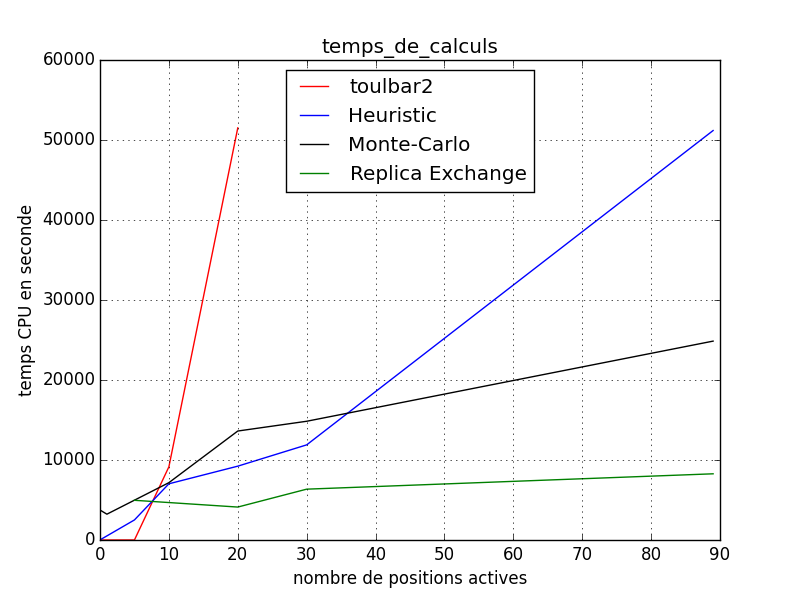
\includegraphics[width=12cm]{resultats/comparaisons/graphe/temps_de_calculs.png} &
      \end{tabular}
      
      \caption{Temps d'occupation du processeur selon le nombre de positions actives.}
      \label{temps_CPU}
    \end{figure}
    
    
    \clearpage
    \section{Les tests} 
   \subsection{Tous les résidus actif} 


   \subsubsection{Les meilleures énergies} 

    \begin{table}[h]
      \centering

      \begin{tabular}{|c|c|c|c|c|c|c|c|c|c|}

        \hline
        Protéine & h & MC3 & MC43 & RE1 & RE2 & RE5 & RE3 & RE32 & RE4 \\
        \hline
        1A81 & -521 & -538 & -522 & -525 & -520 & -520 & -514 & -512 & -518 \\
        1ABO & -272 & -274 & -268 & -273 & -269 & -273 & -268 & -271 & -272 \\
        1BM2 & -484 & -500 & -486 & -488 & -481 & -489 & -478 & -476 & -486 \\
        1CKA & -252 & -258 & -249 & -259 & -251 & -251 & -247 & -246 & -249 \\
        1G9O & -428 & -435 & -428 & -429 & -421 & -430 & -428 & -425 & -428 \\
        1M61 & -480 & -493 & -479 & -483 & -480 & -481 & -480 & -480 & -480 \\
        1O4C & -535 & -545 & -531 & -536 & -529 & -536 & -527 & -524 & -532 \\
        1R6J & -407 & -419 & -414 & -415 & -409 & -411 & -409 & -408 & -414 \\
        2BYG & -457 & -469 & -454 & -461 & -456 & -460 & -456 & -454 & -462 \\
  
        \hline

      \end{tabular}      
      \caption{les meilleures énergies pour tous les résidus actifs}
      \label{tab_best_ener_all}      
    \end{table}


   \begin{figure}[t]
     \centering
     \begin{tabular}{cc}
       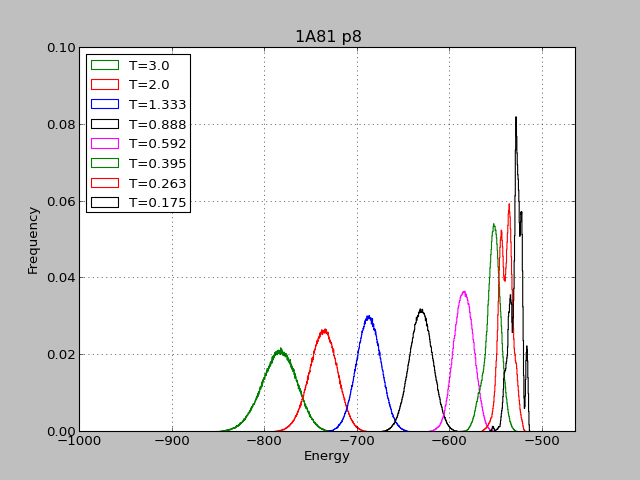
\includegraphics[width=12cm]{resultats/comparaisons/graphe/1A81_casa-p8.png} &
     \end{tabular}
     
     \caption{Distribution des énergies selon la température (protocole RE3).}
     \label{Distrib_E_RE3}
   \end{figure}


   \begin{figure}[t]
     \centering
     \begin{tabular}{cc}
       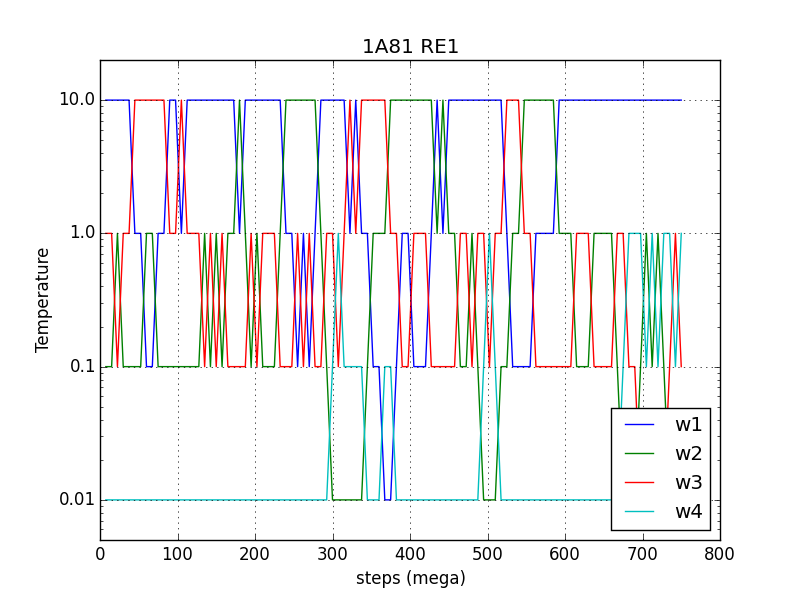
\includegraphics[width=8.45cm]{resultats/comparaisons/graphe/1A81-RE1-T_traj.png} &
       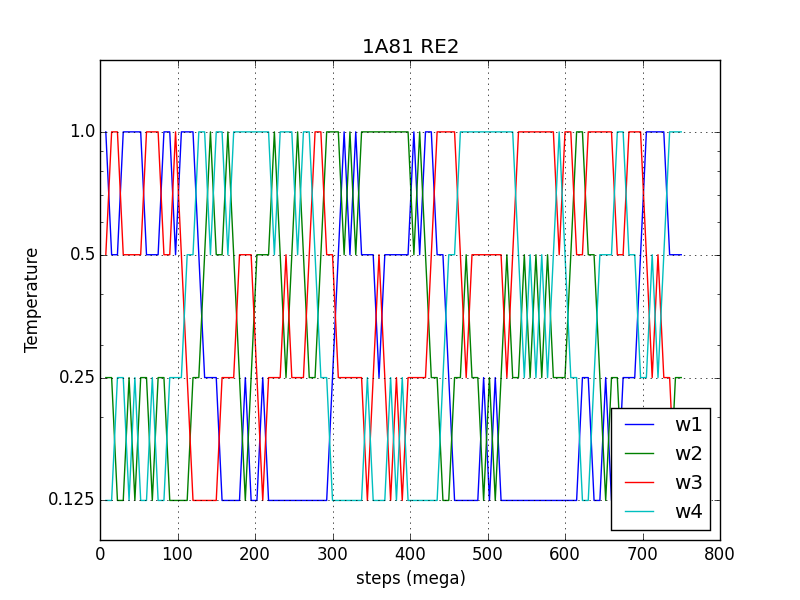
\includegraphics[width=8.45cm]{resultats/comparaisons/graphe/1A81-RE2-T_traj.png} \\
       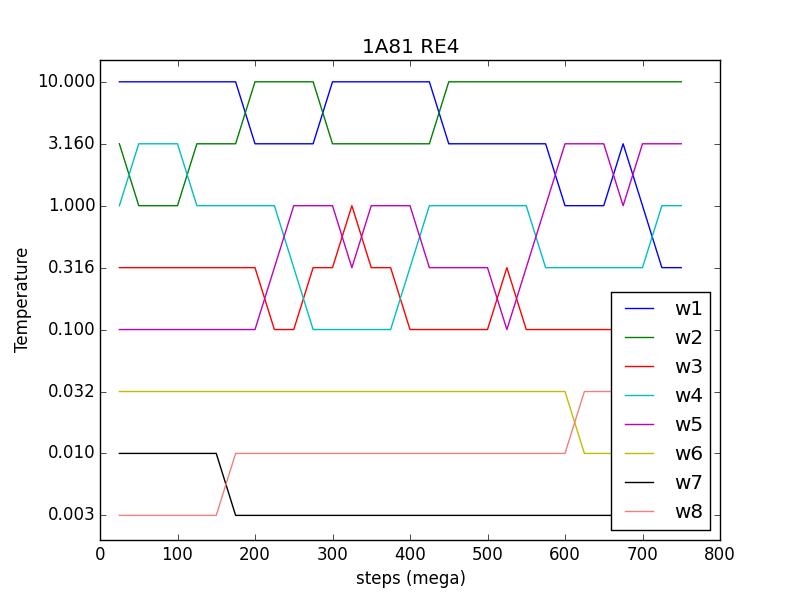
\includegraphics[width=8.45cm]{resultats/comparaisons/graphe/1A81-RE4-T_traj.png} &
       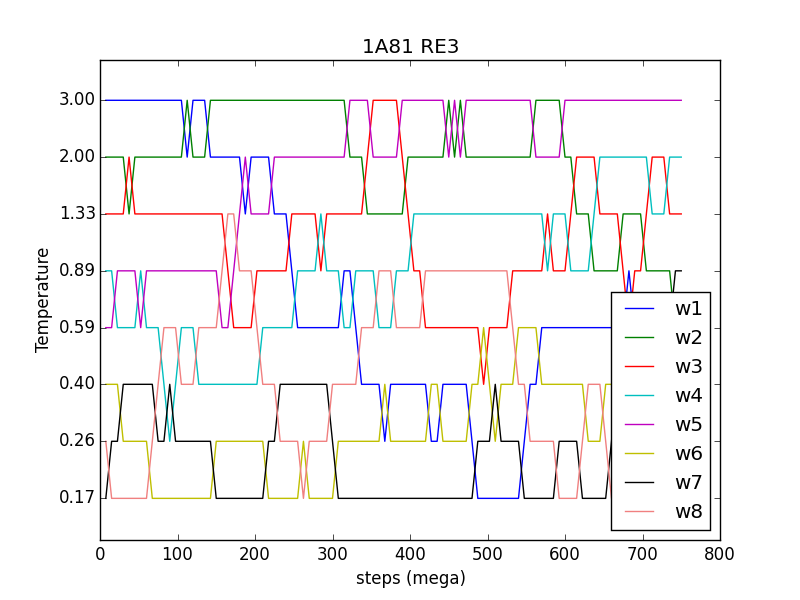
\includegraphics[width=8.45cm]{resultats/comparaisons/graphe/1A81-RE3-T_traj.png} \\
     \end{tabular}
     \caption{Variation de la température au court de la trajectoire de chaque marcheur (protocole RE1).}
     \label{TRAJ_T}
   \end{figure}

    \clearpage

   \begin{figure}[t]
     \centering
     \begin{tabular}{cc}
       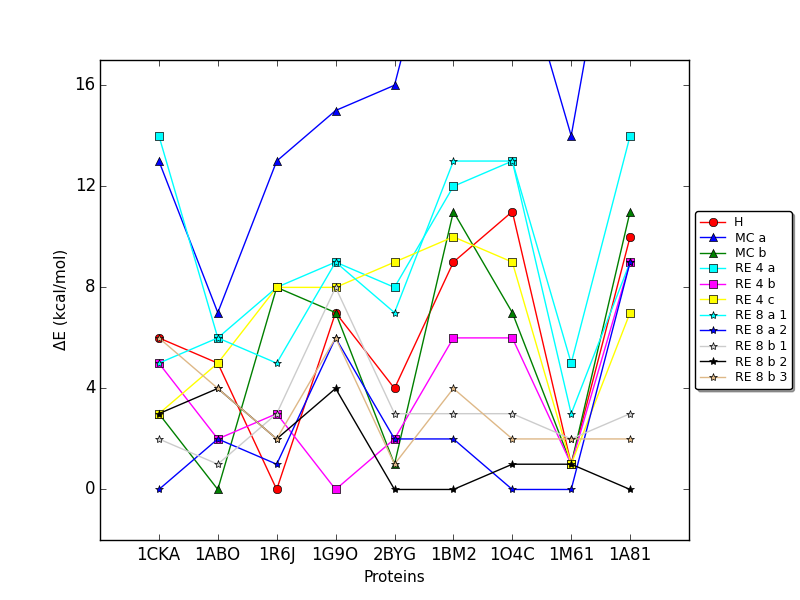
\includegraphics[width=18cm]{resultats/comparaisons/graphe/best_all.png} \\
     \end{tabular}
     \caption{Tous les protocoles.}
     \label{TRAJ_T}
   \end{figure}


    \clearpage


   \begin{figure}[t]
     \centering
     \begin{tabular}{cc}
       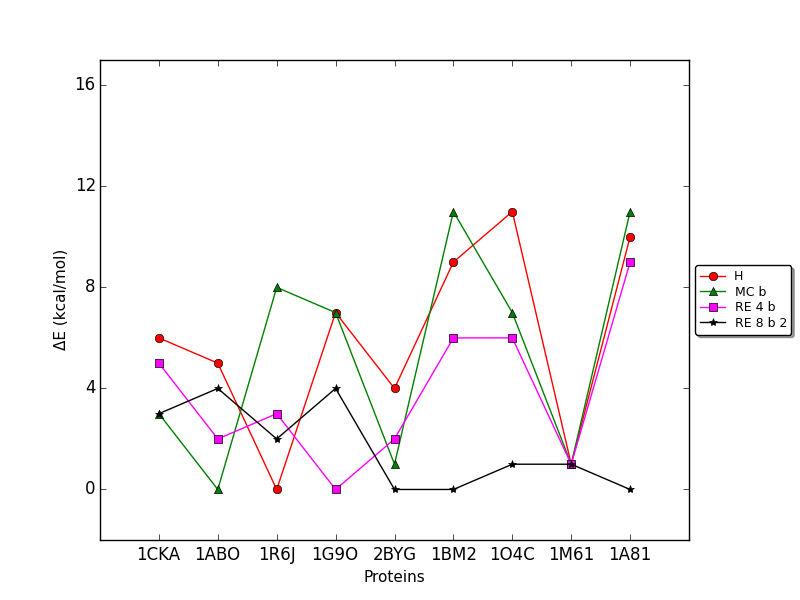
\includegraphics[width=8cm]{resultats/comparaisons/graphe/best_by_cat.png} &
       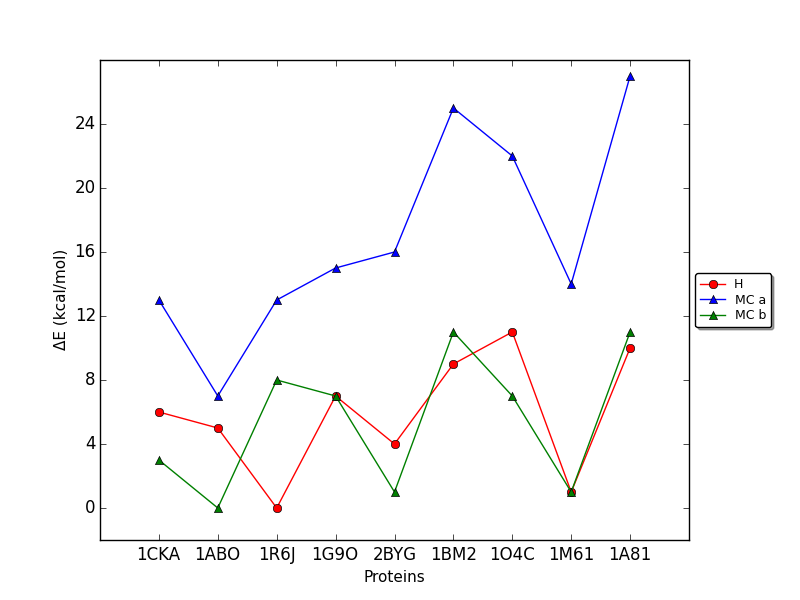
\includegraphics[width=8cm]{resultats/comparaisons/graphe/best_MC+H.png} \\
       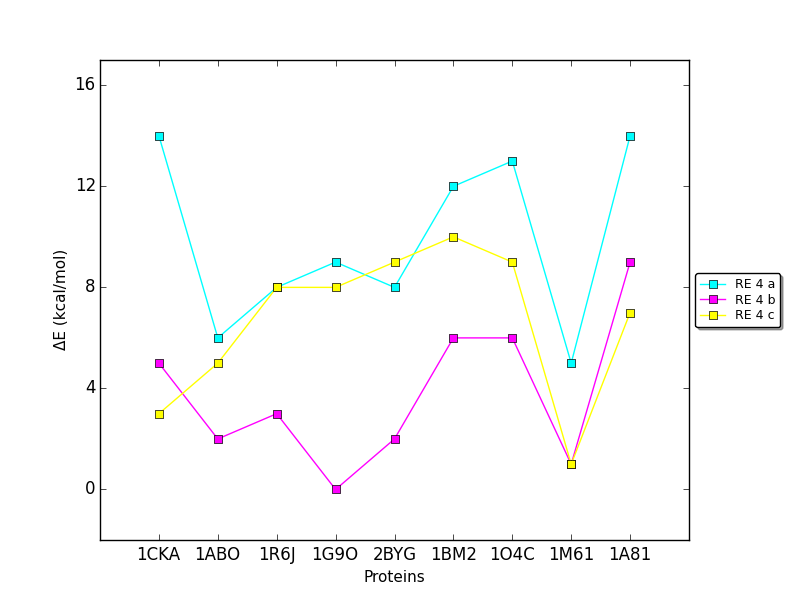
\includegraphics[width=8cm]{resultats/comparaisons/graphe/best_RE4.png} &
       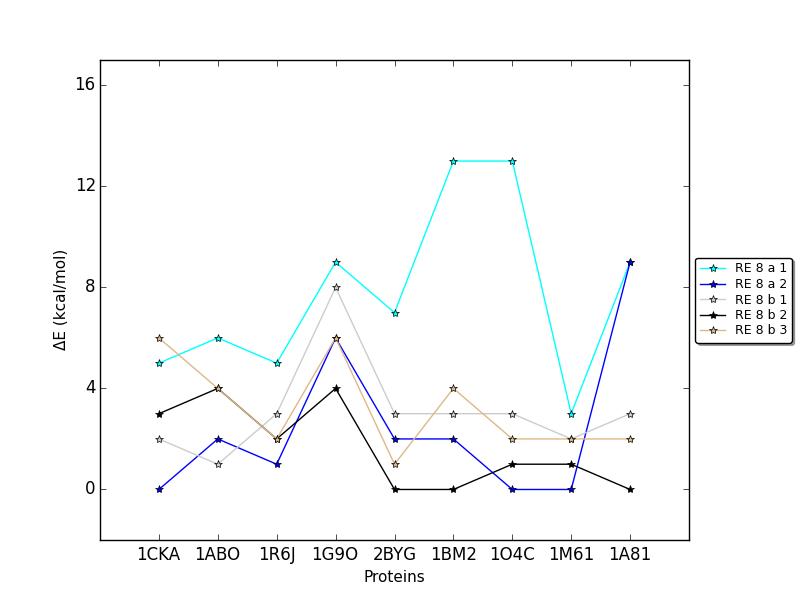
\includegraphics[width=8cm]{resultats/comparaisons/graphe/best_RE8.png} \\
     \end{tabular}
     \caption{Variation de la température au court de la trajectoire de chaque marcheur (protocole RE1).}
     \label{TRAJ_T}
   \end{figure}


    \clearpage

   \subsection{Avec des résidus gelés}
 
   \subsubsection{Séquence native}

 
    \begin{table}[h]
      \centering

      \begin{tabular}{|c|c|c|c|c|c|c|}

        \hline
        Protéine & GMEC & H- & MC0 & MC4- \\
        \hline
        1A81 & -585.1365 & 0 & -0.2547 & 0 \\
        1ABO & -320.1798 & 0 & 0 & 0 \\
        1BM2 & -553.5532 & 0 & -0.0564 & -0.0121 \\
        1CKA & -319.2787 & 0 & 0 & 0 \\
        1G9O & -481.1175 & 0 & -0.1394 & 0 \\
        1M61 & -555.9140 & 0 & 0 & 0 \\
        1O4C & -591.2115 & 0 & 0 & -0.1250 \\
        1R6J & -454.9340 & 0 & 0 & 0 \\
        2BYG & -507.0165 & 0 & 0 & 0 \\        
        \hline


      \end{tabular}      
      \caption{L’énergie du GMEC et la différence avec les autres protocoles.Tous les résidus sont gelés}
      \label{tab_best_ener_no_active}      
    \end{table}


   \subsubsection{Une position active}


    \begin{table}[h]
      \centering

      \begin{tabular}{|c|c|c|}


        \hline
        Position & GMEC & MC4- \\
        \hline
        14 & -584.4693 & -0.0405 \\
        39 & -584.7378 & -0.0111 \\
        55 & -584.0477 & -0.0012 \\
        60 & -583.7763 & -0.0140 \\
        66 & -592.3835 & -0.0347 \\
        70 & -583.8950 & -0.0348 \\
        71 & -588.5916 & -0.0247 \\
        76 & -583.3815 & -0.0248 \\
        79 & -582.8485 & -0.0406 \\
        86 & -584.1412 & -0.0248 \\
        101 & -583.8406 & -0.0248 \\
        105 & -583.0197 & -0.0248 \\
        107 & -582.2241 & -0.0248 \\

        \hline


      \end{tabular}      
      \caption{Liste des échecs pour 1A81}
      \label{tab_best_ener_no_active}      
    \end{table}


    \begin{table}[h]
      \centering

      \begin{tabular}{|c|c|c|}


        \hline
        Position & GMEC & MC4- \\
        \hline
        2 & -553.3134 & -0.0040 \\
        3 & -553.5532 & -0.0121 \\
        5 & -553.0932 & -0.0179 \\
        6 & -553.5532 & -0.0121 \\
        8 & -556.1917 & -0.0148 \\
        10 & -551.4990 & -0.0149 \\
        11 & -551.8859 & -0.0149 \\
        12 & -550.8152 & -0.0148 \\
        13 & -553.4829 & -0.0451 \\
        14 & -553.5532 & -0.0121 \\
        15 & -553.5532 & -0.0121 \\
        17 & -553.5532 & -0.0121 \\
        18 & -553.0880 & -0.0121 \\
        19 & -553.5532 & -0.0270 \\
        20 & -553.0003 & -0.0121 \\
        21 & -553.5532 & -0.0121 \\
        22 & -553.1769 & -0.0121 \\
        29 & -553.5532 & -0.0121 \\
        34 & -553.5532 & -0.0270 \\
        36 & -555.3358 & -0.0317 \\
        37 & -553.5532 & -0.0121 \\
        41 & -553.5076 & -0.0121 \\
        46 & -552.9056 & -0.0149 \\
        49 & -553.5532 & -0.0121 \\
        51 & -553.5532 & -0.0179 \\
        55 & -551.8384 & -0.0121 \\
        56 & -553.5532 & -0.0121 \\
        57 & -561.0695 & -0.0121 \\
        58 & -553.5532 & -0.0121 \\
        62 & -553.5532 & -0.0121 \\
        65 & -553.5532 & -0.0121 \\
        66 & -551.2026 & -0.0179 \\
        68 & -552.6182 & -0.0148 \\
        70 & -553.5532 & -0.0121 \\
        72 & -552.2724 & -0.0121 \\
        73 & -553.5532 & -0.0121 \\
        75 & -553.5532 & -0.0179 \\
        77 & -553.0234 & -0.0466 \\
        80 & -553.5532 & -0.0121 \\
        81 & -553.5532 & -0.0121 \\
        82 & -548.0641 & -0.0121 \\
        83 & -553.5532 & -0.0121 \\
        85 & -550.1884 & -0.0122 \\
        86 & -552.7375 & -0.0148 \\
        87 & -550.6139 & -0.0121 \\
        90 & -552.8601 & -0.0009 \\
        91 & -553.5532 & -0.0121 \\
        92 & -553.5532 & -0.0121 \\
        93 & -553.2772 & -0.0148 \\
        94 & -553.3207 & -0.0251 \\
        96 & -553.5532 & -0.0121 \\
        \hline


      \end{tabular}      
      \caption{Liste des échecs pour 1BM2}
      \label{tab_best_ener_no_active}      
    \end{table}




    \begin{table}[h]
      \centering

      \begin{tabular}{|c|c|c|}


        \hline
        Position & GMEC & MC4- \\
        \hline
        17 & -316.1693 & -0.0109 \\

\hline
      \end{tabular}      
      \caption{Liste des échecs pour 1CKA}
      \label{tab_echec_1CKA_1}      
    \end{table}

    \begin{table}[h]
      \centering

      \begin{tabular}{|c|c|c|}

        \hline
        \hline
        Position & GMEC & MC4 \\
        \hline
        58 & -561.9469 & -0.0138 \\
        
        \hline

      \end{tabular}      
      \caption{Liste des échecs pour 1M61}
      \label{tab_echec1M61__1}      
    \end{table}
    

    \begin{table}[h]
      \centering
      
      \begin{tabular}{|c|c|c|}
        



        \hline
        Position & GMEC & MC4- \\
        \hline
        1 & -591.2115 & -0.1380 \\
        2 & -591.2115 & -0.1250 \\
        3 & -591.2115 & -0.1250 \\
        4 & -590.7216 & -0.0319 \\
        5 & -590.5458 & -0.1071 \\
        6 & -591.2115 & -0.1521 \\
        7 & -590.7923 & -0.1429 \\
        8 & -591.2115 & -0.1250 \\
        9 & -591.2115 & -0.1728 \\
        10 & -591.2115 & -0.2572 \\
        11 & -589.9443 & -0.2489 \\
        12 & -591.1022 & -0.1137 \\
        13 & -589.9867 & -0.0535 \\
        14 & -591.2115 & -0.1250 \\
        15 & -589.4899 & -0.0436 \\
        16 & -591.2115 & -0.1521 \\
        17 & -590.4460 & -0.0557 \\
        18 & -589.0053 & -0.1366 \\
        19 & -590.7580 & -0.0348 \\
        20 & -591.2115 & -0.1250 \\
        21 & -591.2115 & -0.1600 \\
        22 & -591.2115 & -0.1250 \\
        23 & -590.5249 & -0.1530 \\
        24 & -590.7262 & -0.0630 \\
        25 & -591.2115 & -0.1250 \\
        26 & -591.2115 & -0.1250 \\
        27 & -590.8058 & -0.1194 \\
        28 & -591.2115 & -0.1250 \\
        29 & -591.2115 & -0.1571 \\
        30 & -590.5207 & -0.0221 \\
        31 & -590.5507 & -0.0530 \\
        32 & -591.2115 & -0.1571 \\
        33 & -591.2115 & -0.1234 \\
        34 & -590.7486 & -0.1258 \\
        35 & -591.2115 & -0.0378 \\
        36 & -589.1510 & -0.0974 \\
        37 & -591.0133 & -0.0941 \\
        38 & -589.2126 & -0.2743 \\
        39 & -589.0387 & -0.1890 \\
        40 & -590.8793 & -0.0883 \\
        41 & -589.4209 & -0.0409 \\
        42 & -591.2115 & -0.1250 \\
        43 & -587.9420 & -0.1315 \\
        44 & -589.8470 & -0.0595 \\
        45 & -591.2115 & -0.1712 \\
        46 & -588.8346 & -0.2668 \\
        47 & -589.9117 & -0.2773 \\
        48 & -588.6520 & -0.2625 \\
        49 & -591.2115 & -0.2120 \\
        50 & -590.6561 & -0.0807 \\
        51 & -591.1249 & -0.2986 \\
        52 & -589.7127 & -0.2734 \\
        53 & -590.7224 & -0.3012 \\
        54 & -590.8735 & -0.3615 \\
        55 & -588.6242 & -0.2007 \\
        56 & -591.2115 & -0.2120 \\
        57 & -591.2115 & -0.1250 \\
        58 & -590.6832 & -0.0743 \\
        59 & -591.2115 & -0.0378 \\
        60 & -591.1842 & -0.1082 \\
        61 & -590.6996 & -0.1272 \\
        62 & -595.8620 & -0.0899  \\
        63 & -591.2115 & -0.0974 \\
        64 & -588.8836 & -0.1014 \\
        65 & -591.2115 & -0.1571 \\
        66 & -590.1420 & -0.1533 \\
        67 & -587.5415 & -0.0433 \\
        68 & -590.1771 & -0.1541 \\
        69 & -591.2115 & -0.1250 \\
        70 & -590.4684 & -0.1066 \\
        71 & -591.2115 & -0.1250 \\
        72 & -591.2115 & -0.1311 \\
        73 & -591.2115 & -0.1250 \\
        74 & -588.7096 & -0.1169 \\
        75 & -590.2437 & -0.0505 \\
        76 & -591.2115 & -0.1521 \\
        78 & -587.6940 & -0.0821 \\
        79 & -589.9770 & -0.1380 \\
        80 & -591.1165 & -0.0661 \\
        81 & -590.2528 & -0.1229 \\
        82 & -589.8459 & -0.0724 \\
        83 & -590.2079 & -0.0513 \\
        84 & -591.2095 & -0.0433 \\
        85 & -590.8011 & -0.1154 \\
        87 & -590.7787 & -0.0744 \\
        88 & -590.2860 & -0.0857 \\
        89 & -591.2115 & -0.1250 \\
        90 & -590.2493 & -0.1084 \\
        91 & -589.5602 & -0.0694 \\
        92 & -589.3260 & -0.1838 \\
        93 & -590.4697 & -0.0188 \\
        94 & -587.4192 & -0.3392 \\
        95 & -590.0201 & -0.2937 \\
        96 & -590.6312 & -0.2723 \\
        97 & -595.0049 & -0.2864 \\
        98 & -590.0135 & -0.2013 \\
        99 & -589.7855 & -0.2932 \\
        100 & -591.2115 & -0.2120 \\
        101 & -591.2115 & -0.2120 \\
        102 & -591.2115 & -0.2572 \\
        103 & -595.4168 & -0.1277 \\
        104 & -589.9208 & -0.3581 \\
        
        \hline


      \end{tabular}      
      \caption{Liste des échecs pour 1O4C}
      \label{tab_echec1O4C__1}      
    \end{table}

    \begin{table}[h]
      \centering

      \begin{tabular}{|c|c|c|}


        \hline
        Position & GMEC & MC4- \\
        \hline
         4 & -453.4484 & -0.0155  \\
        20 & -452.6464 & -0.0114 \\
        32 & -454.9340 & -0.0092 \\
        68 & -454.4856 & -0.0060 \\
        73 & -454.7809 & -0.0155 \\
        77 & -454.1344 & -0.0155 \\
        79 & -453.4729 & -0.0155 \\
        
        \hline


      \end{tabular}      
      \caption{Liste des échecs pour 1R6J }
      \label{tab_echec1R6J__1}      
    \end{table}


    \begin{table}[h]
      \centering

      \begin{tabular}{|c|c|c|}

        \hline
        Position & GMEC & MC4- \\
        \hline
        1 & -505.2910 & -0.0132 \\
        3 & -506.7960 & -0.0254 \\
        4 & -505.5800 & -0.0023 \\
        5 & -506.8732 & -0.0948 \\
        49 & -505.5183 & -0.0135 \\
        59 & -507.0165 & -0.0100 \\
        85 & -506.6217 & -0.0101 \\
        88 & -505.2286 & -0.0097 \\
        95 & -506.3195 & -0.0131 \\

        \hline


      \end{tabular}      
      \caption{Liste des échecs pour 2BYG }
      \label{tab_echec2BYG__1}      
    \end{table}


   \subsubsection{Cinq positions actives}


    \begin{table}[h]
      \centering

      \begin{tabular}{|c|c|c|c|c|}


        \hline
        \hline
        Protéine & GMEC & H & MC4 & RE3 \\
        \hline
        1A81 1 & -579.3989 & 0 & 0 &  \\
        1A81 2 & -575.2254 & 0 & 0 &  \\
        1A81 3 & -582.7452 & 0 & 0 &  \\
        1A81 4 & -569.9383 & 0 & -5.3443 & 0 \\
        1A81 5 & -591.8143 & 0 & 0 &  \\
        1ABO 1 & -315.4497 & 0 & 0 &  \\
        1ABO 2 & -316.6637 & 0 & 0 &  \\
        1ABO 3 & -307.4824 & 0 & 0 &  \\
        1ABO 4 & -313.7710 & 0 & 0 &  \\
        1ABO 5 & -313.5695 & 0 & 0 &  \\
        1BM2 1 & -548.2341 & 0 & 0 &  \\
        1BM2 2 & -554.8135 & 0 & 0 &  \\
        1BM2 3 & -557.8629 & 0 & 0 &  \\
        1BM2 4 & -544.9791 & 0 & 0 &  \\
        1BM2 5 & -550.2956 & 0 & -0.0121 &  \\
        1CKA 1 & -315.0859 & 0 & 0 &  \\
        1CKA 2 & -309.7692 & 0 & 0 &  \\
        1CKA 3 & -317.3820 & 0 & 0 &  \\
        1CKA 4 & -314.8550 & 0 & 0 &  \\
        1CKA 5 & -312.0405 & -0.0001 & -0.0001 &  \\
        1G9O 1 & -469.9540 & 0 & 0 &  \\
        1G9O 2 & -476.4094 & 0 & 0 &  \\
        1G9O 3 & -479.7190 & 0 & 0 &  \\
        1G9O 4 & -478.9513 & 0 & 0 &  \\
        1G9O 5 & -480.7260 & 0 & 0 &  \\
        1M61 1 & -557.6647 & 0 & 0 &  \\
        1M61 2 & -546.9587 & 0 & 0 &  \\
        1M61 3 & -553.0731 & 0 & 0 &  \\
        1M61 4 & -555.0885 & 0 & 0 &  \\
        1M61 5 & -554.6356 & 0 & 0 &  \\
        1O4C 1 & -584.4267 & 0 & -0.0655 &  \\
        1O4C 2 & -584.8989 & 0 & -0.1437 &  \\
        1O4C 3 & -588.4971 & 0 & -0.1164 &  \\
        1O4C 4 & -587.7129 & 0 & -0.1400 &  \\
        1O4C 5 & -587.6514 & 0 & -0.1168 &  \\
        1R6J 1 & -444.5018 & 0 & 0 &  \\
        1R6J 2 & -449.3043 & 0 & -0.9421 & 0 \\
        1R6J 3 & -453.1139 & 0 & 0 &  \\
        1R6J 4 & -453.1139 & 0 & 0 &  \\
        1R6J 5 & -454.9340 & 0 & 0 &  \\
        2BYG 1 & -500.7946 & 0 & -0.0150 &  \\
        2BYG 2 & -506.2319 & 0 & 0 &  \\
        2BYG 3 & -506.8744 & 0 & -0.0131 &  \\
        2BYG 4 & -504.5135 & 0 & 0 &  \\
        2BYG 5 & -506.0052 & 0 & 0 &  \\

        \hline




 \end{tabular}      
 \caption{Résultats 5 position actives}
 \label{tab_echec2BYG__1}      
\end{table}


   \subsubsection{Dix positions actives}


    \begin{table}[h]
      \centering

      \begin{tabular}{|c|c|c|c|c|}


        \hline
        Protéine & GMEC & H & MC4 & RE32 \\
        \hline
        1A81 1 & -583.9354 & 0 & 0 & \\
        1A81 2 & -581.7802 & 0 & 0 & \\
        1A81 3 & -587.4392 & -0.0001 & -0.1595 & \\
        1A81 4 & -589.1322 & 0 & -0.0317 & \\
        1A81 5 & -578.2558 & 0 & -0.0563 & \\
        1ABO 1 & -309.1670 & -0.0675 & -0.9054 & \\
        1ABO 2 & -308.8387 & 0 & 0 & \\
        1ABO 3 & -303.8520 & 0 & 0 & \\
        1ABO 4 & -310.0087 & 0 & -0.0128 & \\
        1ABO 5 & -301.6727 & 0 & 0 & \\
        1BM2 1 & -549.8638 & 0 & -0.0950 & \\
        1BM2 2 & -541.5944 & 0 & 0 & \\
        1BM2 3 & -543.7434 & 0 & 0 & \\
        1BM2 4 & -549.0453 & 0 & 0 & \\
        1BM2 5 & -544.1447 & 0 & -0.1082 & \\
        1CKA 1 & -305.8477 & 0 & 0 & \\
        1CKA 2 & -309.9886 & 0 & 0 & \\
        1CKA 3 & -304.6618 & 0 & 0 & \\
        1CKA 4 & -302.4894 & 0 & 0 & \\
        1CKA 5 & -299.2329 & -0.2859 & -3.2525 & 0 \\
        1G9O 1 & -466.6764 & 0 & 0 & \\
        1G9O 2 & -478.8797 & 0 & 0 & \\
        1G9O 3 & -477.2503 & -0.1366 & 0 & \\
        1G9O 4 & -470.6458 & 0 & 0 & \\
        1G9O 5 & -464.8659 & 0 & -3.9599 & \\
        1M61 1 & -550.0699 & 0 & -0.0776 & \\
        1M61 2 & -538.6026 & -3.5105 & -4.5062 & 0.3215 \\
        1M61 3 & -552.2673 & 0 & 0 & \\
        1M61 4 & -550.0553 & 0 & 0 & \\
        1M61 5 & -553.6559 & 0 & -0.0432 & \\
        1O4C 1 & -587.4665 & 0 & -0.1121 & \\
        1O4C 2 & -585.8545 & 0 & -0.1046 & \\
        1O4C 3 & -580.3505 & 0 & -0.1519 & \\
        1O4C 4 & -587.1548 & 0 & -0.1545 & \\
        1O4C 5 & -590.2650 & 0 & -0.1753 & \\
        1R6J 1 & -448.8351 & 0 & -2.4022 & -2.3986 \\
        1R6J 2 & -448.4631 & 0 & -1.0398 & \\
        1R6J 3 & -450.3950 & 0 & -0.0106 & \\
        1R6J 4 & -451.7211 & 0 & 0 & \\
        1R6J 5 & -450.9943 & 0 & -0.0162 & \\
        2BYG 1 & no & -505.6397 & -0.0337 & \\
        2BYG 2 & -504.7389 & 0 & 0 & \\
        2BYG 3 & -504.3048 & 0 & -0.0833 & \\
        2BYG 4 & -504.3466 & 0 & -0.2149 & \\
        2BYG 5 & -491.6095 & 0 & 0 & \\
        
        \hline


 \end{tabular}      
 \caption{Résultats 10 positions actives }
 \label{tab_echec2BYG__1}      
\end{table}


   \subsubsection{Vingt et trente positions actives}



    \begin{table}[h]
      \centering

      \begin{tabular}{|c|c|c|c|c|c|c|c|c|}


        \hline
        \multicolumn{5}{|c|}{10 positions actives}  & \multicolumn{4}{|c|}{20 positions actives} \\
        \hline
        Protéine & GMEC & H & MC & RE & GMEC & H & MC & RE \\
        \hline
        1A81 1 & -583.9354 & 0 & 0 & & -566.9106 & 0 & -0.3275 & -.3851 \\             
        1A81 2 & -581.7802 & 0 & 0 & & -564.6618 & -0.1705 & -2.4355 & -1.0069 \\    
        1A81 3 & -587.4392 & -0.0001 & -0.1595 & & -572.9780 & 0 & -0.4640 & -.6186 \\       
        1A81 4 & -589.1322 & 0 & -0.0317 & & -570.3480 & -0.3568 & -0.5128 & -.6991 \\     
        1A81 5 & -578.2558 & 0 & -0.0563 & & -571.2480 & -0.7658 & -0.5088 & -.6991 \\     
        1ABO 1 & -309.1670 & -0.0675 & -0.9054 & & -299.6592 & -0.1205 & -1.1159 & -0.2153 \\    
        1ABO 2 & -308.8387 & 0 & 0 & & no & -298.3854 & 0 & 0 \\ 
        1ABO 3 & -303.8520 & 0 & 0 & & no & -298.3854 & 0 & 0 \\            
        1ABO 4 & -310.0087 & 0 & -0.0128 & & no & -297.8545 & -0.0076 & 0 \\          
        1ABO 5 & -301.6727 & 0 & 0 & & no & -297.8009 & -0.9483 & -.9483 \\       
        1BM2 1 & -549.8638 & 0 & -0.0950 & &   -526.0936 & 0 & -0.0619 & -.1584 \\        
        1BM2 2 & -541.5944 & 0 & 0 & & no & -525.3588 & -0.0725 & -.0143 \\       
        1BM2 3 & -543.7434 & 0 & 0 & & -534.3860 & -0.0230 & -0.4763 & -.2898 \\     
        1BM2 4 & -549.0453 & 0 & 0 & & no & -526.8307 & -2.5883 & -0.0789 \\       
        1BM2 5 & -544.1447 & 0 & -0.1082 & & -535.3334 & -0.2396 & -0.3746 & -.3746 \\     
        1CKA 1 & -305.8477 & 0 & 0 & & -295.6311 & 0 & 0 & 0\\  
        1CKA 2 & -309.9886 & 0 & 0 & & -295.8571 & 0 & 0 & 0 \\ 
        1CKA 3 & -304.6618 & 0 & 0 & & -293.8687 & 0 & 0 & 0 \\ 
        1CKA 4 & -302.4894 & 0 & 0 & & no & -293.8687 & 0 & 0 \\ 
        1CKA 5 & -299.2329 & -0.2859 & -3.2525 & 0 & no & -293.4203 & 0 & 0 \\ 
        1G9O 1 & -466.6764 & 0 & 0 & & no & -451.4604 & -1.2525 & -1.2525 \\       
        1G9O 2 & -478.8797 & 0 & 0 & & no & -453.2355 & -0.2487 & -.1915 \\       
        1G9O 3 & -477.2503 & -0.1366 & 0 & & no & -453.2474 & -0.2177 & -.1915 \\       
        1G9O 4 & -470.6458 & 0 & 0 & & no & -456.3751 & -0.2275 & -.1455 \\       
        1G9O 5 & -464.8659 & 0 & -3.9599 & & no & -456.7331 & -0.1455 & -.1455 \\       
        1M61 1 & -550.0699 & 0 & -0.0776 & & -528.0700 & 0 & 0 & 0 \\ 
        1M61 2 & -538.6026 & -3.5105 & -4.5062 & 0.3215 & -528.7653 & 0 & 0 & 0 \\ 
        1M61 3 & -552.2673 & 0 & 0 & & -530.0684 & 0 & 0 & 0 \\ 
        1M61 4 & -550.0553 & 0 & 0 & & -534.5248 & 0 & 0 & 0 \\ 
        1M61 5 & -553.6559 & 0 & -0.0432 & & -548.0096 & 0 & -0.2521 & -0.1345 \\          
        1O4C 1 & -587.4665 & 0 & -0.1121 & & no & -.2878 & -.0103 & -574.0634 \\        
        1O4C 2 & -585.8545 & 0 & -0.1046 & & no & -574.8584 & -0.1963 & -.3175 \\       
        1O4C 3 & -580.3505 & 0 & -0.1519 & & -573.6314 & 0 & -0.3461 & -.0997 \\        
        1O4C 4 & -587.1548 & 0 & -0.1545 & & -575.8667 & 0 & -0.3640 & -.1382 \\        
        1O4C 5 & -590.2650 & 0 & -0.1753 & & no & -573.3479 & -0.1141 & -.2206 \\       
        1R6J 1 & -448.8351 & 0 & -2.4022 & -0.3986 & -440.7417 & 0 & -0.2604 & -.2002 \\        
        1R6J 2 & -448.4631 & 0 & -1.0398 & & -437.2537 & 0 & -0.0071 & -.0183 \\        
        1R6J 3 & -450.3950 & 0 & -0.0106 & & -439.4335 & 0 & -0.0537 & -.0732 \\        
        1R6J 4 & -451.7211 & 0 & 0 & & -439.9135 & 0 & -0.0537 & -.0732 \\        
        1R6J 5 & -450.9943 & 0 & -0.0162 & & -438.0222 & 0 & -0.0735 & -.0244 \\        
        2BYG 1 & no & -505.6397 & -0.0337 & & -496.2991 & 0 & -3.1878 & -.0257 \\        
        2BYG 2 & -504.7389 & 0 & 0 & & -494.8723 & 0 & -0.0524 & -.0826 \\        
        2BYG 3 & -504.3048 & 0 & -0.0833 & & -494.8723 & 0 & -1.3564 & -.0826 \\        
        2BYG 4 & -504.3466 & 0 & -0.2149 & & -495.9213 & 0 & -0.1968 & -.6022 \\        
        2BYG 5 & -491.6095 & 0 & 0 & & no & -497.5123 & -0.0933 & -.0386 \\       
    
    \hline


 \end{tabular}      
 \label{tab_echec_10_20}      
\end{table}





   \subsection{Etude au voisinnage de GMECs}


    \begin{table}[h]
      \centering

      \begin{tabular}{|c|c|c|c|c|}

        Protéine & nb seq (GMEC + 1) & rang H &rang MC & rang RE \\
        \hline

        1CKA 3 &  67668 & 1 & 1 & \\
        1CKA 4 &  4647 & 1 & 1 & \\
        1CKA 5 &  255 &  10 & 182638 & 1 \\
        1G9O 3 &  435881 & 24 & 1 \\
        1G9O 4 &  354476 & 1 & 1 \\
        1G9O 5 &  61 & 1 & 897112 & 1 \\
        1M61 2 &  261467 &  & \\
        1M61 3 &  11199152 & 1 & 1 &\\
        1M61 4 &  16417603  & 1 & 1 & \\
        \hline


 \end{tabular}      
 \caption{Résultats 30 positions actives }
 \label{tab_echec2BYG__1}      
\end{table}


    \clearpage
    
    \begin{figure}[h]
      \centering
      \begin{tabular}{c} 
        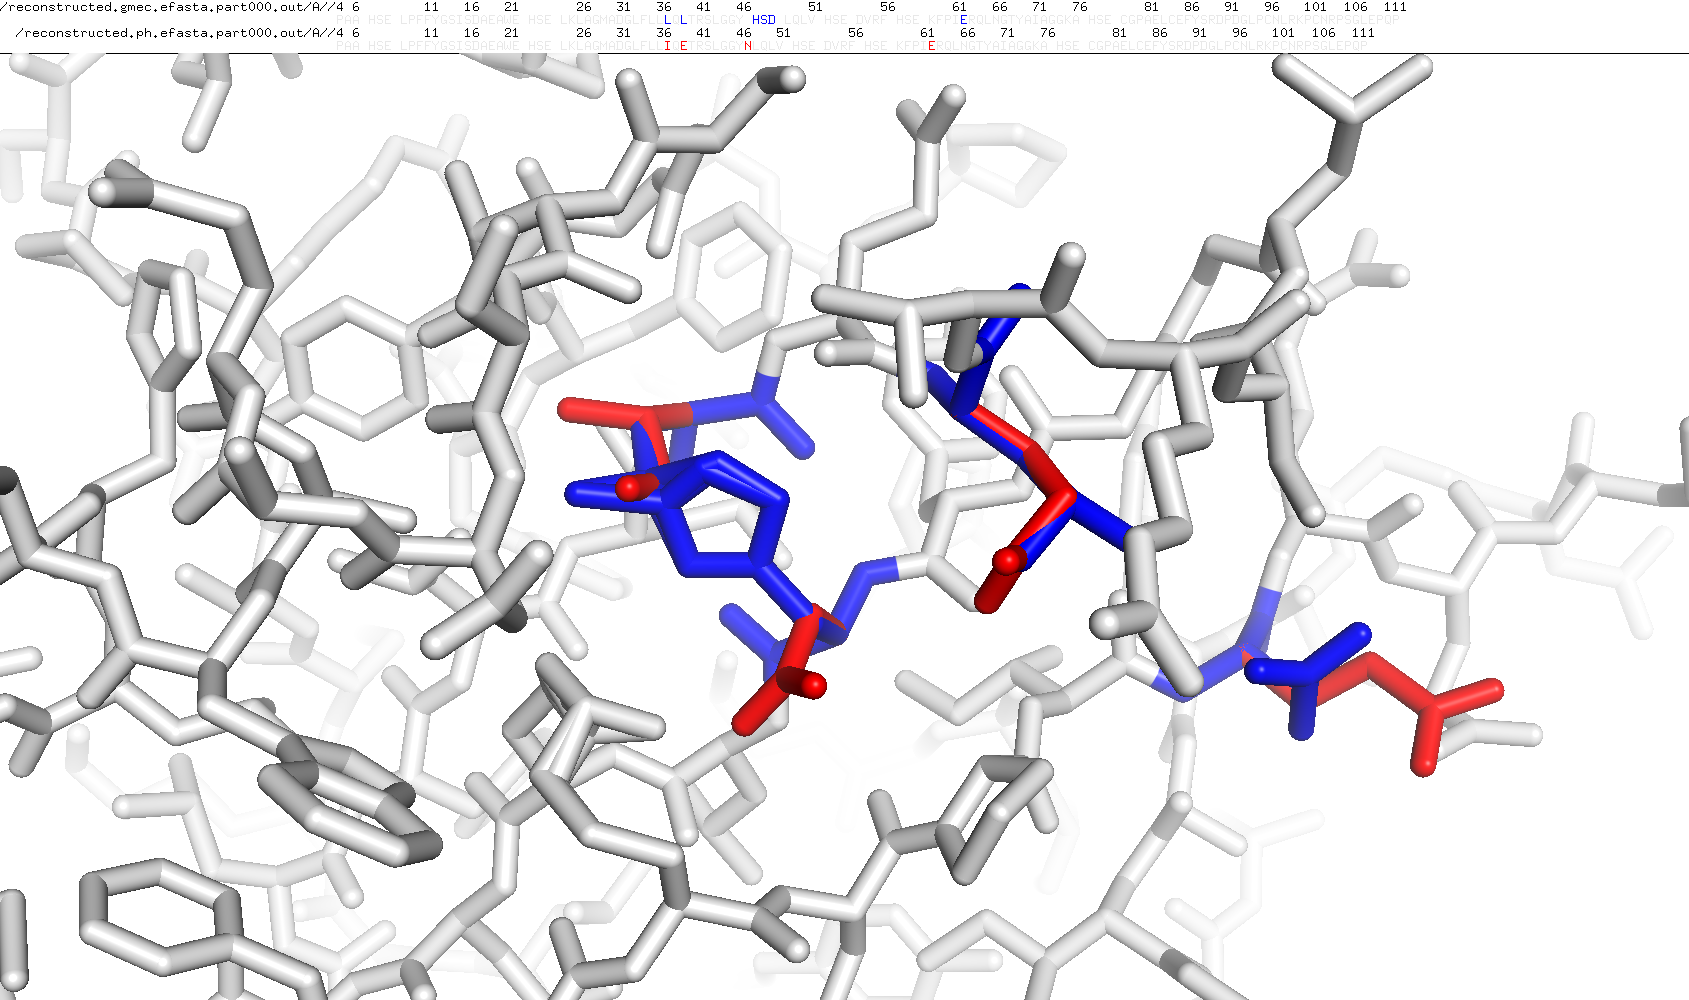
\includegraphics[width=14cm]{resultats/comparaisons/image/1M61_2_gmec_vs_ph.png} 
      \end{tabular}
      
      \caption{test: 1M61 2, GMEC vs H}
      \label{temps_CPU}
    \end{figure}
    
    
    
    \begin{figure}[h]
      \centering
      \begin{tabular}{c} 
        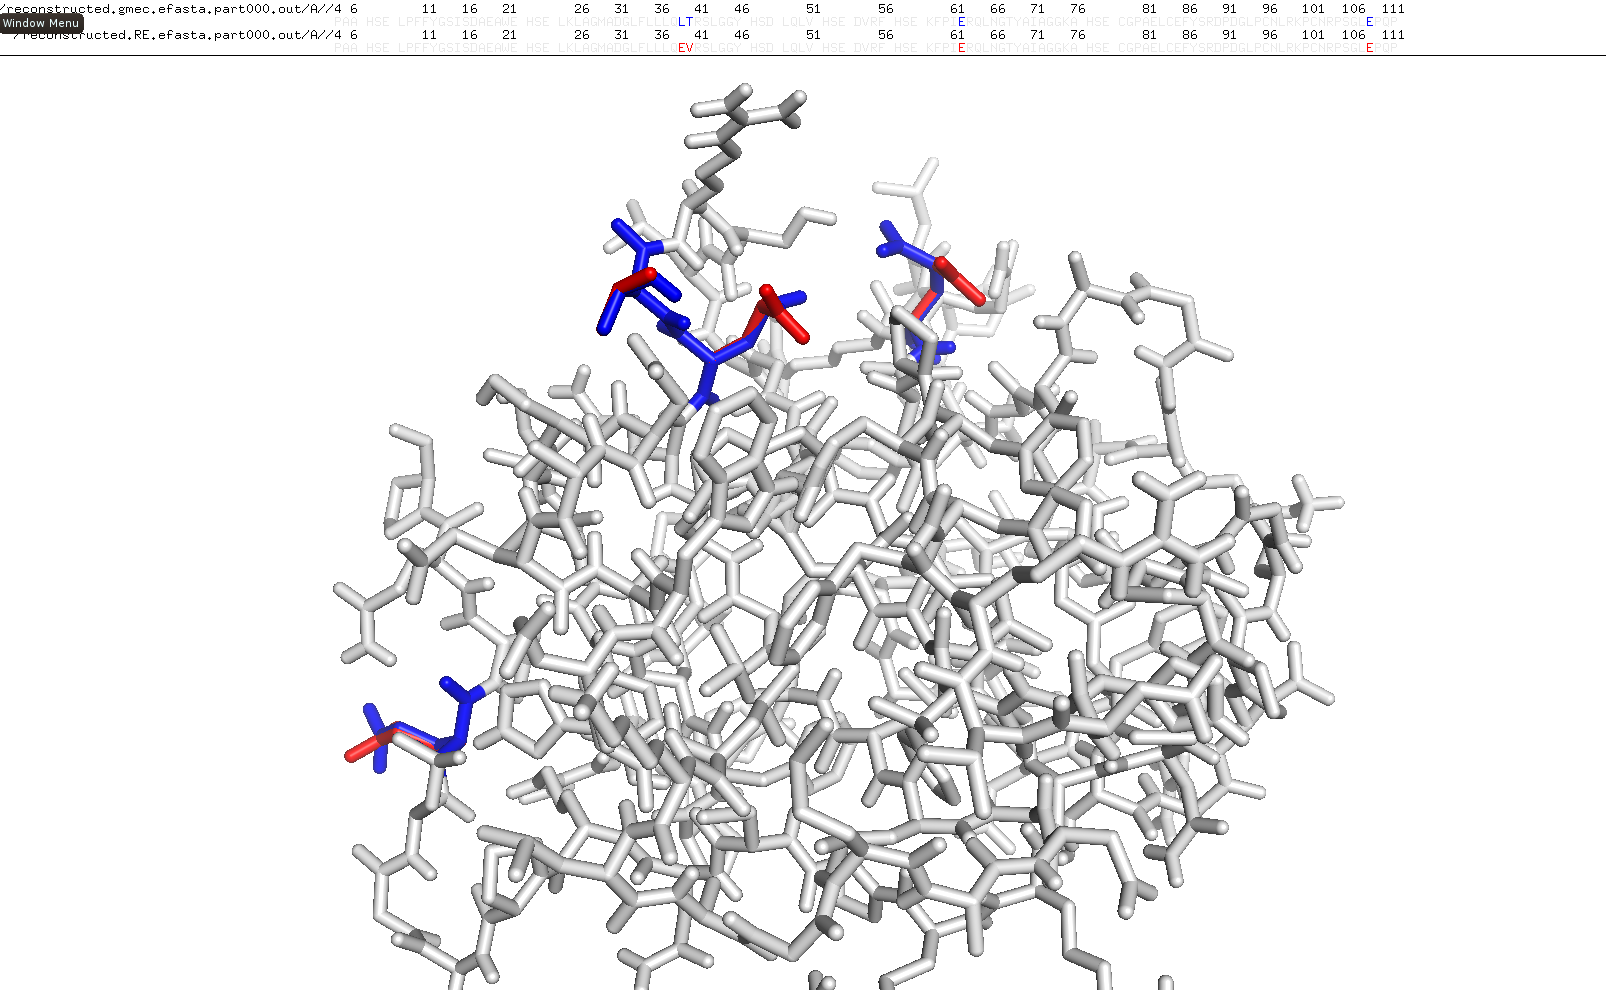
\includegraphics[width=14cm]{resultats/comparaisons/image/1M61_2_gmec_vs_RE.png} 
      \end{tabular}
      
      \caption{test: 1M61 2, GMEC vs RE}
      \label{temps_CPU}
    \end{figure}
    
    
    

    \begin{figure}[h]
      \centering
      \begin{tabular}{c} 
        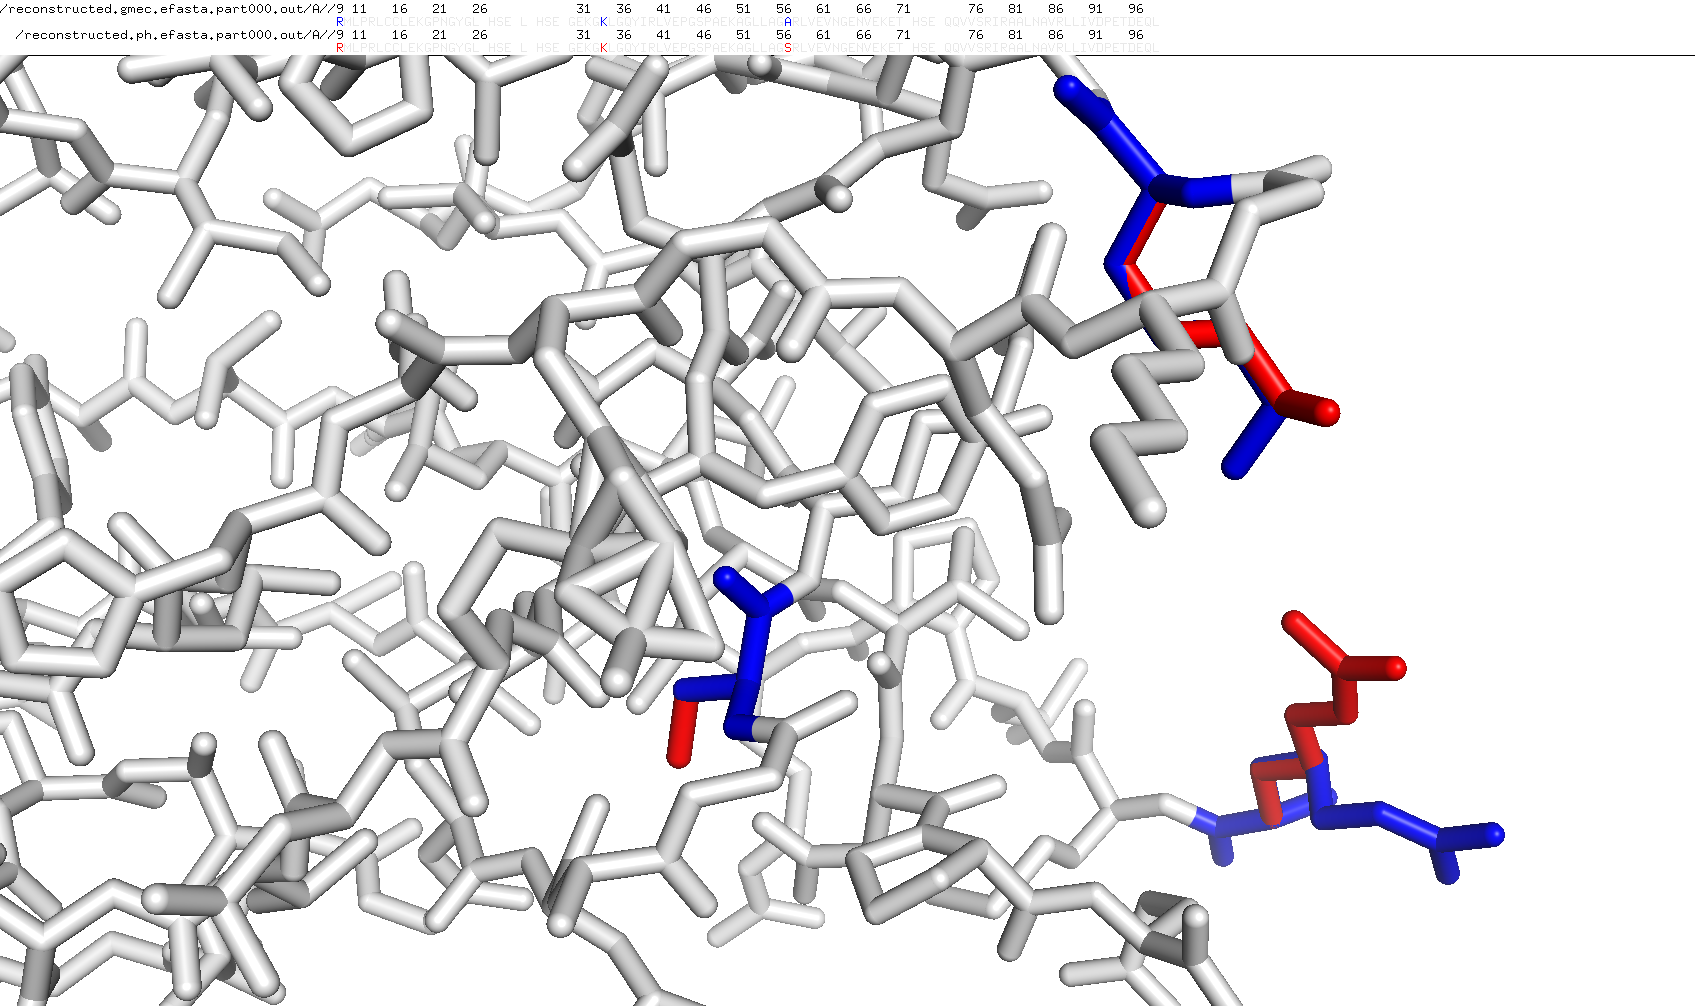
\includegraphics[width=14cm]{resultats/comparaisons/image/1G9O_3_gmec_vs_ph.png} 
      \end{tabular}
      
      \caption{test: 1G9O 3, GMEC vs H}
      \label{temps_CPU}
    \end{figure}
    
    
    \begin{figure}[h]
      \centering
      \begin{tabular}{c} 
        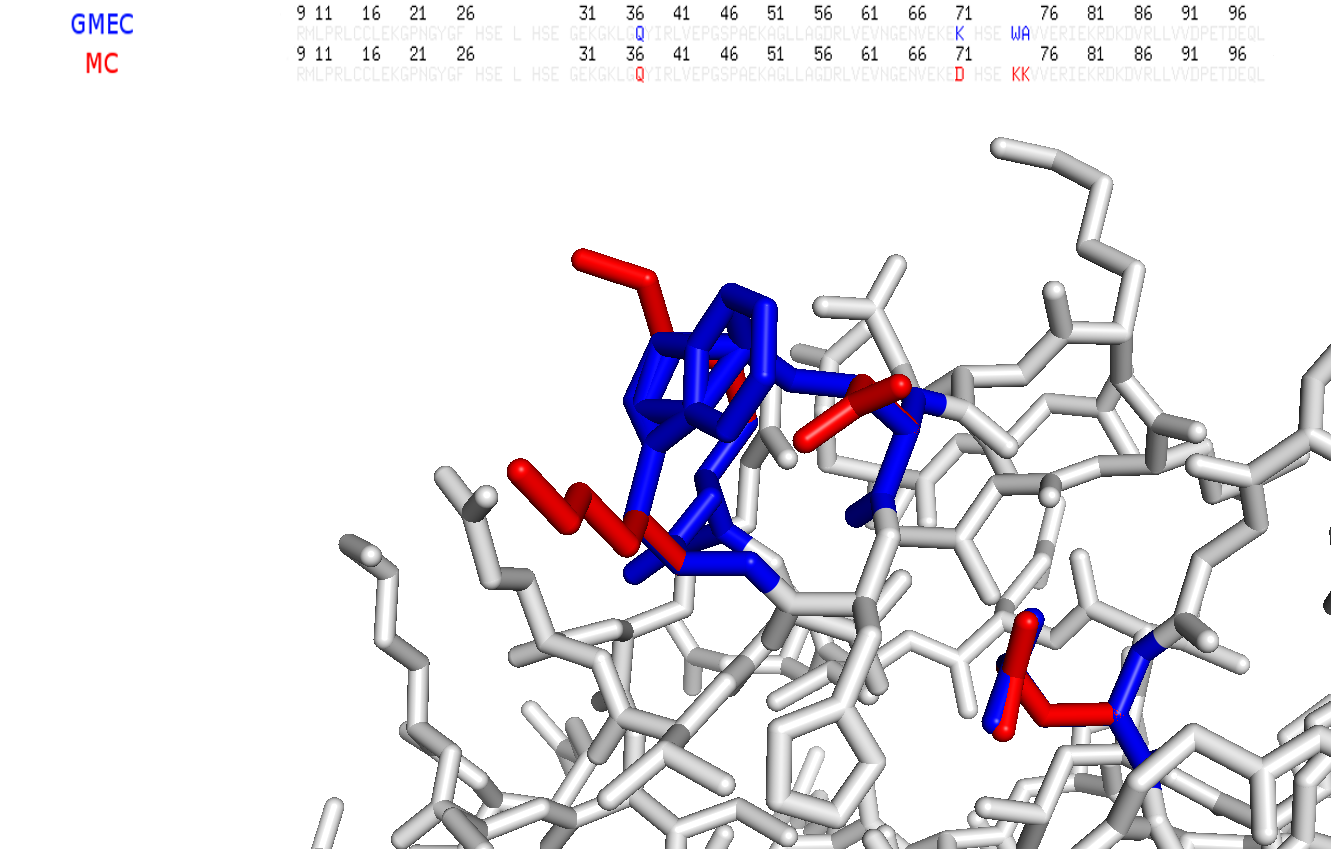
\includegraphics[width=14cm]{resultats/comparaisons/image/1G9O_5_gmec_vs_MC.png} 
      \end{tabular}
      
      \caption{test: 1G9O 5, GMEC vs MC}
      \label{temps_CPU}
    \end{figure}
    
    \begin{figure}[h]
      \centering
      \begin{tabular}{c} 
        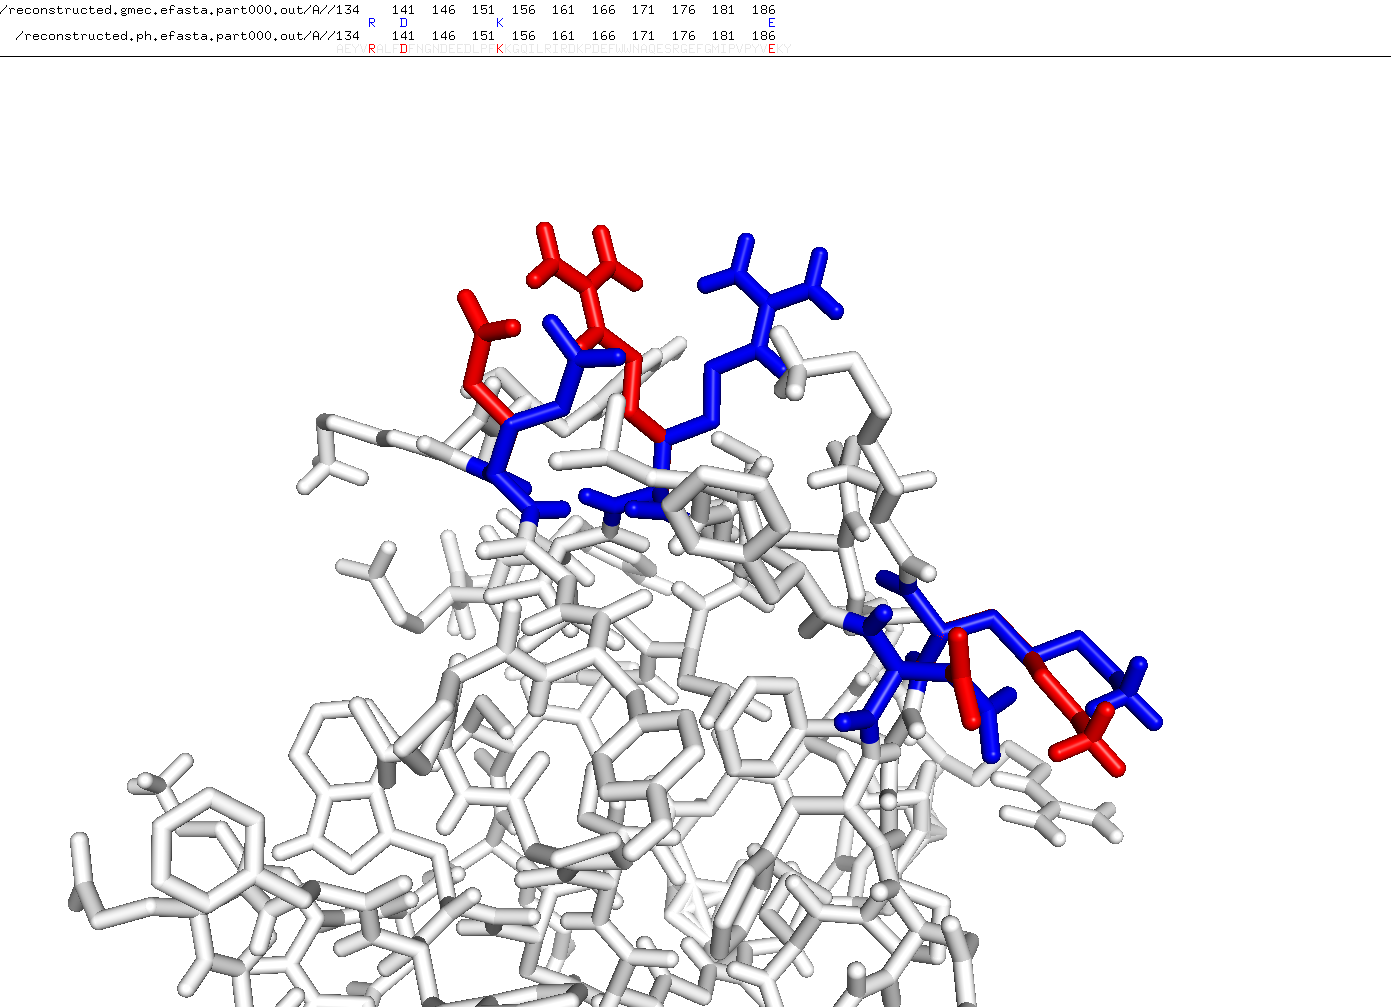
\includegraphics[width=14cm]{resultats/comparaisons/image/1CKA_5_gmec_vs_ph.png} 
      \end{tabular}
      
      \caption{test: 1CKA 5, GMEC vs H}
      \label{temps_CPU}
    \end{figure}
    
    

    \begin{figure}[h]
      \centering
      \begin{tabular}{c} 
        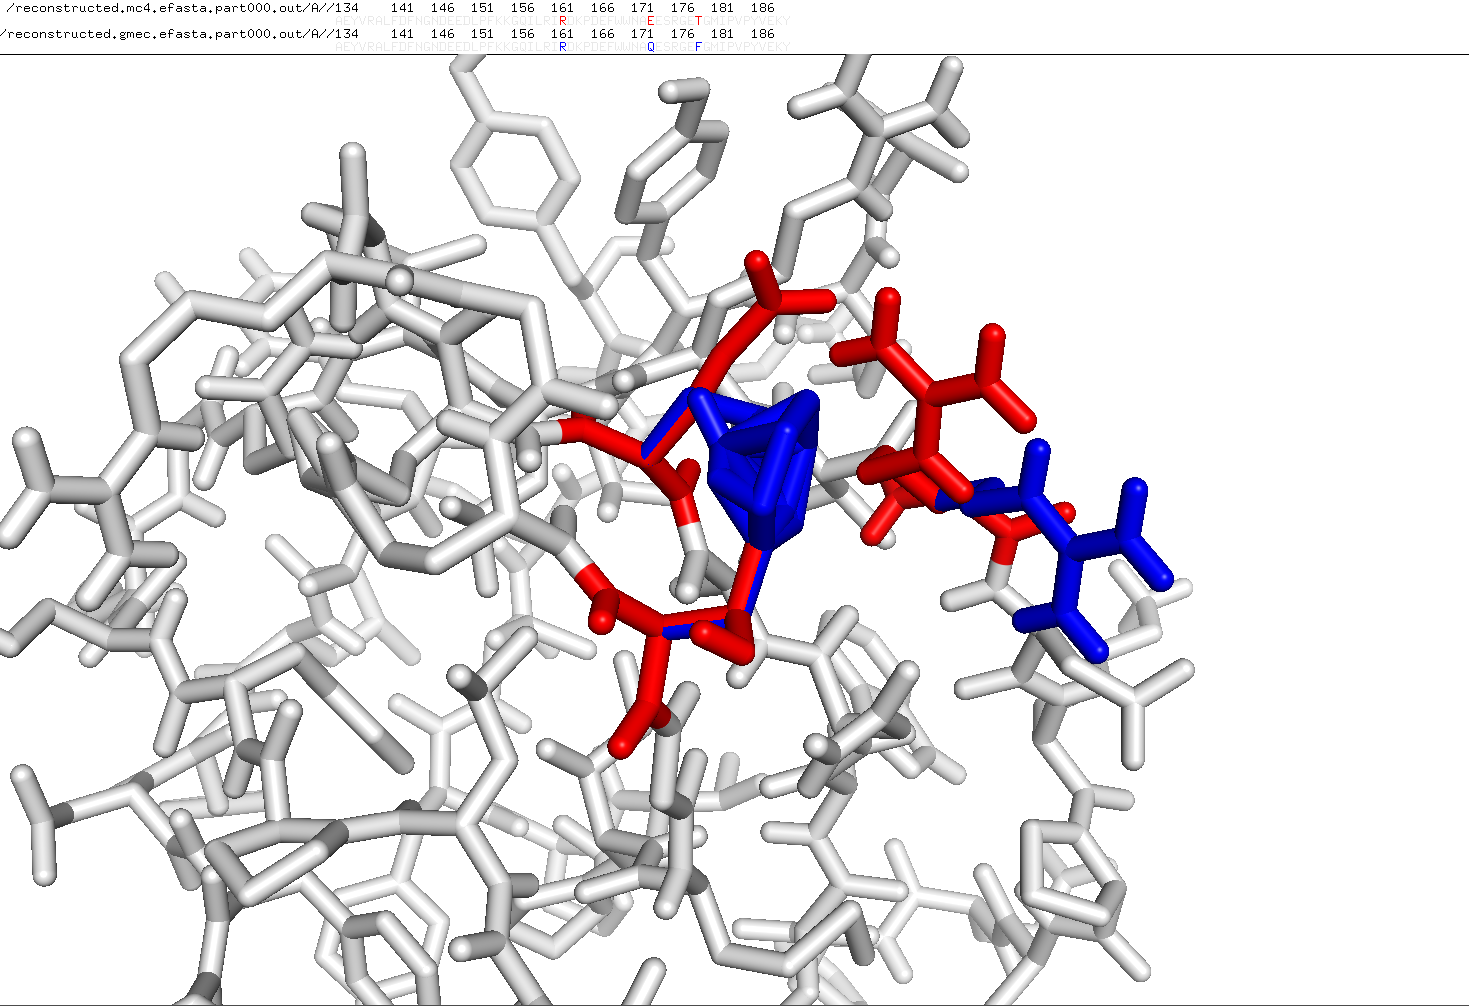
\includegraphics[width=14cm]{resultats/comparaisons/image/1CKA_5_gmec_vs_MC.png} 
      \end{tabular}
      
      \caption{test: 1CKA 5, GMEC vs MC}
      \label{temps_CPU}
    \end{figure}
    
    
    \clearpage





   \subsection{Résultats Superfamily}


    \begin{table}[h]
           \raggedleft

      \begin{tabular}{|c|c|c|c|c|c|}

        \hline
        Protein & Match/seq size & Superfamily Evalue & superfamily success & Family Evalue & family success\\
        \hline
        1A81 & no & & & & \\
        1ABO & 51/58 & 4.4e-4 & 100\% & 2.8e-3 & 100\% \\
        1BM2 & 78/98 & 4.2e-5 & 100\% & 2.6e-3 & 100\% \\
        1CKA & 40/57 & 1.1e-5 & 100\% & 3.4e-3. & 100\% \\
        1G9O & 79/91 & 7.0e-7 & 100\% & 2.5e-3 & 100\%  \\
        1M61 & 97/109 & 7.2e-7 & 100\% & 2.6e-4 &  100\% \\
        1O4C & 95/104 & 2.1e-4 & 100\% & 4.5e-3 &  100\% \\
        1R6J & 74/82 & 9.8e-6 & 100\% & 4.6e-3 &  100\% \\
        2BYG & 59/97 & 1.4e-5 & 100\% & 7.1e-3 &  100\% \\

        \hline


 \end{tabular}      


 \label{tab_echec2BYG__1}       
\end{table}



    \clearpage


    \begin{table}[h]
      \centering

      \begin{tabular}{|c|c|c|c|c|}


        \hline
        Protein & GMEC & H & MC & RE \\
        \hline
        1CKA 3 & -304.6618 & 0 & 0 & \\
        1CKA 4 & -302.4894 & 0 & 0 & \\
        1CKA 5 & -299.2329 & -0.2859 & -3.2525 & 0 \\
        1G9O 3 & -477.2503 & -0.1366 & 0 & \\
        1G9O 4 & -470.6458 & 0 & 0 & \\
        1G9O 5 & -464.8659 & 0 & -3.9599 &  0 \\
        1M61 1 & -550.0699 & 0 & -0.0776 & \\
        1M61 2 & -538.6026 & -3.5105 & -4.5062 & 0.3215 \\
        1M61 5 & -553.6559 & 0 & -0.0432 & \\
        
        \hline


 \end{tabular}      
 \label{tab_1}      
\end{table}


    \begin{table}[h]
      \centering

      \begin{tabular}{|c|c|c|c|c|c|c|}


        \hline
        Protein & seq-rot nb gmec+1 & H rank  & MC rank  & seq nb gmec+1 & H mut nb & MC mut nb \\
        \hline
        1CKA 3 & 67669 & 1 & 1 & 227 & 0 & 0 \\
        1CKA 4 & 4649 & 1 & 1 & 498 & 0 & 0 \\
        1CKA 5 & 1388 & 78 & no & 77 & 0 & 2 \\
        1G9O 3 & 354559 & 23 & 1 & 63 & 1 & 0 \\
        1G9O 4 & 22639 & 1 & 1 & 381 & 0 & 0 \\
        1G9O 5 & 8658395 & 1 & no &  11 & 0 & 3 \\
        1M61 1 & 11199153 & no & no & 21 & 3 & 7 \\
        1M61 2 & 11199153 & 1 & 1 & 88 & 0 & 0 \\
        1M61 5 & 16417604 & 1 & 1 & 83 & 0 & 0 \\
        
        \hline


 \end{tabular}      
 \label{tab_2}      
\end{table}




    \clearpage

   \subsection{Résultats Heuristic (protocoles longs)}


    \begin{table}[h]
      \centering

      \begin{tabular}{|c|c|c|c|c|}

        \hline
        Proteins & GMEC & H & H+ & H++ \\
        \hline
        1ABO 1 & -309.1670 & -0.0675 & -0.0675 & 0 \\
        1CKA 5 & -299.2329 & -0.2859 & -0.0640 & 0 \\
        1G9O 3 & -477.2503 & -0.1366 & 0 & 0 \\
        1M61 2 & -538.6026 & -3.5105 & -2.1673 & -0.0188 \\
        \hline


 \end{tabular}      
 \caption{Résultats pour 3 fois (resp 9 fois ) plus de cycles heuristiques protocole H+ (resp H++)}
 \label{tab_echec2BYG__1}       
\end{table}



    \clearpage

    \clearpage

   \subsection{densité en séquences }



    \begin{figure}[h]
      \centering
      \begin{tabular}{cc} 
        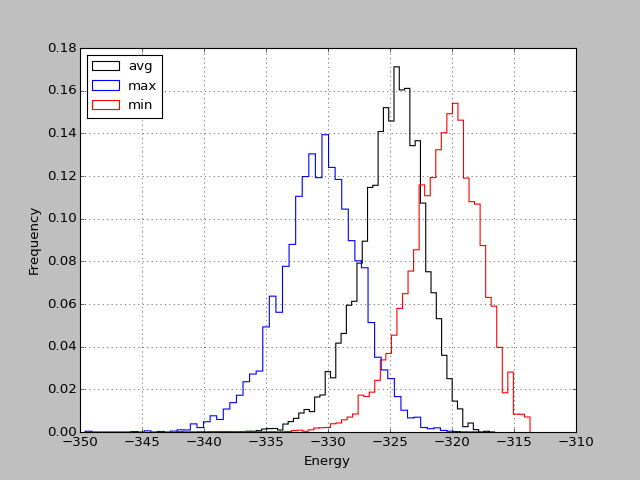
\includegraphics[width=10cm]{resultats/comparaisons/graphe/histo1_aa_Tambiante.png} &
      \end{tabular}
      
      \caption{.}
      \label{temps_CPU}
    \end{figure}


    \begin{figure}[h]
      \centering
      \begin{tabular}{cc} 
        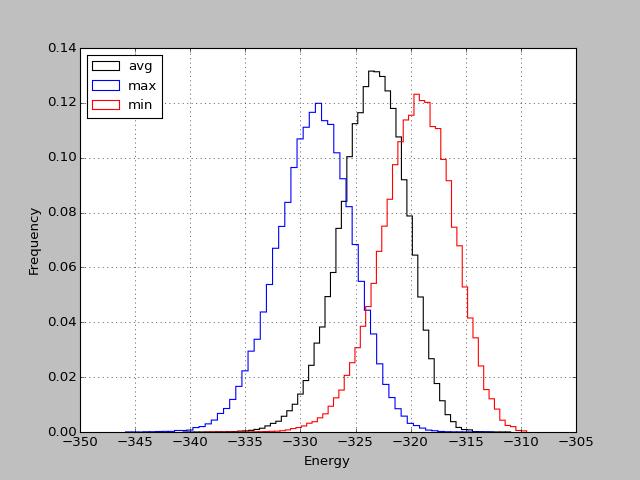
\includegraphics[width=10cm]{resultats/comparaisons/graphe/histo2_aa_Tambiante.png} &
      \end{tabular}
      
      \caption{.}
      \label{temps_CPU}
    \end{figure}

    \clearpage



\chapter{Les Méthodes utilisées}
\label{chap:methodes_pratiques}
 
\section{Section}

XXX

\subsection{Subsection}

XXX

\subsubsection{Subsubsection}

XXX

\paragraph{Paragraph}

XXX

\subparagraph{Subparagraph}

Référence à une équation (Équation~\ref{eq:label_equation}).

\begin{equation}
H \Psi = E \Psi
\label{eq:label_equation}
\end{equation}

\chapter{Résultats des comparaisons}
\label{chap:resultats_comparaisons}

   \section{Les algorithmes} 

   \subsection{Toulbar2} 
   \subsection{l'heuristique} 
   \subsection{Le Monte-Carlo}
   \subsection{Le Replica Exchange}
 

\subparagraph{Subparagraph}

Référence à une table (Table~\ref{tab:label_table}).

\begin{table}[!htbp]
\centering

\caption{Légende de la table}

\vspace{2ex}
\begin{tabular}{lcc}
\hline
Colonne1$^a$ & Colonne2$^b$ & Colonne3$^c$\\
\hline
X1 & X2 & X3\\
Y1 & Y2 & Y3\\
Z1 & Z2 & Z3\\
\hline
\end{tabular}

\bigskip

{\raggedright

$^a$ note1

$^b$ note2

$^c$ note3

}

\label{tab:label_table}
\end{table}



   \section{Les protocoles} 



   \subsection{Les protocoles Monte-Carlo} 
    
    \begin{table}[!htbp]
      \centering

      \begin{tabular}{|l|r|r|c|c|}

        \hline
        Nom & Temp & Traj (mega)& seuil voisin  & Proba \\
        \hline
        MC0   & 0.01  &  6000 & 0 & 0; 1; 0.1; 0   \\  
        MC0-  & 0.01  &   300 & 0 & 0; 1; 0.1; 0   \\  
        MC4   & 0.2   &  6000 & 0 & 0; 1; 0.1; 0   \\          
        MC4-  & 0.2   &   300 & 0 & 0; 1; 0.1; 0   \\ 
        MC42  & 0.2   &  6000 & 0 & 1; 0; 0.1; 0   \\        
        MC42- & 0.2   &   300 & 0 & 1; 0; 0.1; 0   \\   \hline                   

       
      \end{tabular}      
      \caption{Les protocoles Monte-Carlo}
      \label{tab_protoMC}      
    \end{table}

   \subsection{Les protocoles Replica Exchange} 
    
    \begin{table}[!htbp]
      \centering

      \begin{tabular}{|l|l|r|r|r|c|c|}

        \hline
        Nom & marcheurs &Temp & Traj (mega)& seuil voisin  & Proba & swap period (mega)\\
        \hline
        RE1   & 4 & 10<->0.01    &  1500 & 10 & 1; 0; 0.1; 0 &  7.5\\  
        RE2   & 4 & 1<->0.125    &  1500 & 10 & 1; 0; 0.1; 0 &  7.5\\  
        RE2-  & 4 & 1<->0.125    &  250  & 10 & 1; 0; 0.1; 0 &  2.5\\  
        RE22  & 4 & 2<->0.25     &  1500 & 10 & 1; 0; 0.1; 0 &  7.5\\  
        RE3   & 8 & 3<->0.175    &  750  & 10 & 1; 0; 0.1; 0 &  7.5\\
        RE32  & 8 & 3<->0.175    &  750  & 10 & 0; 1; 0.1; 0 &  7.5\\
        RE4   & 8 & 10<->0.00316 &  750  & 10 & 1; 0; 0.1; 0 &  1\\  
        RE42  & 8 & 10<->0.00316 &  750  &  0 & 1; 0; 0.1; 0 &  2.5\\  \hline

      \end{tabular}      
      \caption{Les protocoles Replica Exchange}
      \label{tab_protoRE}      
    \end{table}


   \subsection{Les protocoles Heuristic} 
    
    \begin{table}[!htbp]
      \centering

      \begin{tabular}{|c|r|}

        \hline
        Nom & nombre de cycles \\
        \hline
        h   & 110000 \\  
        h-  & 1100   \\  \hline

      \end{tabular}      
      \caption{Les protocoles Heuristic}
      \label{tab_protoH}      
    \end{table}

    \clearpage
    \subsection{Les temps de calcul} 
    
    \begin{figure}[h]
      \centering
      \begin{tabular}{cc}
        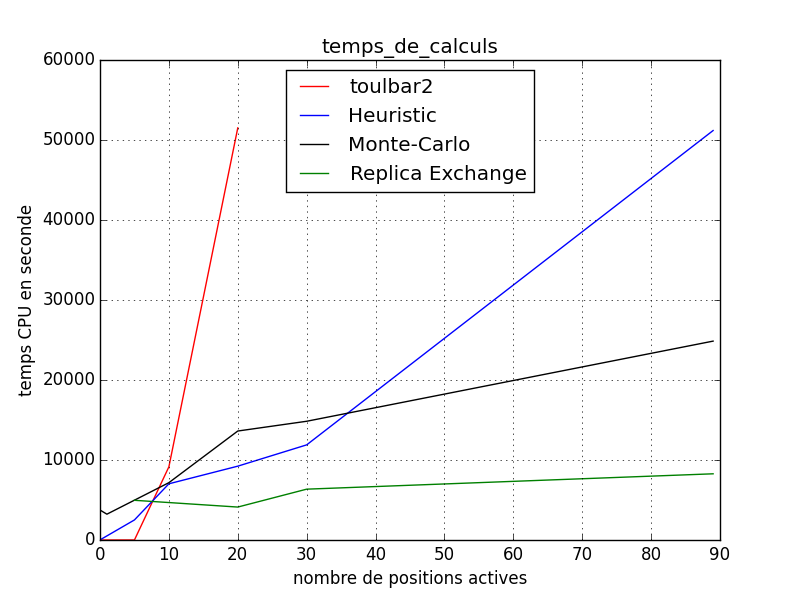
\includegraphics[width=12cm]{resultats/comparaisons/graphe/temps_de_calculs.png} &
      \end{tabular}
      
      \caption{Temps d'occupation du processeur selon le nombre de positions actives.}
      \label{temps_CPU}
    \end{figure}
    
    
    \clearpage
    \section{Les tests} 
   \subsection{Tous les résidus actif} 


   \subsubsection{Les meilleures énergies} 

    \begin{table}[h]
      \centering

      \begin{tabular}{|c|c|c|c|c|c|c|c|c|c|}

        \hline
        Protéine & h & MC3 & MC43 & RE1 & RE2 & RE5 & RE3 & RE32 & RE4 \\
        \hline
        1A81 & -521 & -538 & -522 & -525 & -520 & -520 & -514 & -512 & -518 \\
        1ABO & -272 & -274 & -268 & -273 & -269 & -273 & -268 & -271 & -272 \\
        1BM2 & -484 & -500 & -486 & -488 & -481 & -489 & -478 & -476 & -486 \\
        1CKA & -252 & -258 & -249 & -259 & -251 & -251 & -247 & -246 & -249 \\
        1G9O & -428 & -435 & -428 & -429 & -421 & -430 & -428 & -425 & -428 \\
        1M61 & -480 & -493 & -479 & -483 & -480 & -481 & -480 & -480 & -480 \\
        1O4C & -535 & -545 & -531 & -536 & -529 & -536 & -527 & -524 & -532 \\
        1R6J & -407 & -419 & -414 & -415 & -409 & -411 & -409 & -408 & -414 \\
        2BYG & -457 & -469 & -454 & -461 & -456 & -460 & -456 & -454 & -462 \\
  
        \hline

      \end{tabular}      
      \caption{les meilleures énergies pour tous les résidus actifs}
      \label{tab_best_ener_all}      
    \end{table}


   \begin{figure}[t]
     \centering
     \begin{tabular}{cc}
       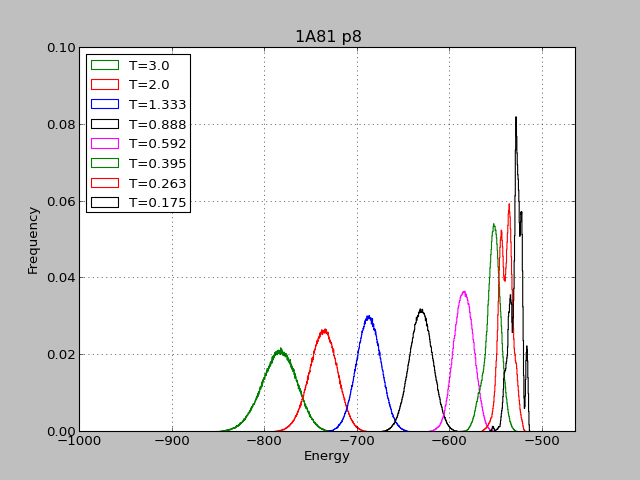
\includegraphics[width=12cm]{resultats/comparaisons/graphe/1A81_casa-p8.png} &
     \end{tabular}
     
     \caption{Distribution des énergies selon la température (protocole RE3).}
     \label{Distrib_E_RE3}
   \end{figure}


   \begin{figure}[t]
     \centering
     \begin{tabular}{cc}
       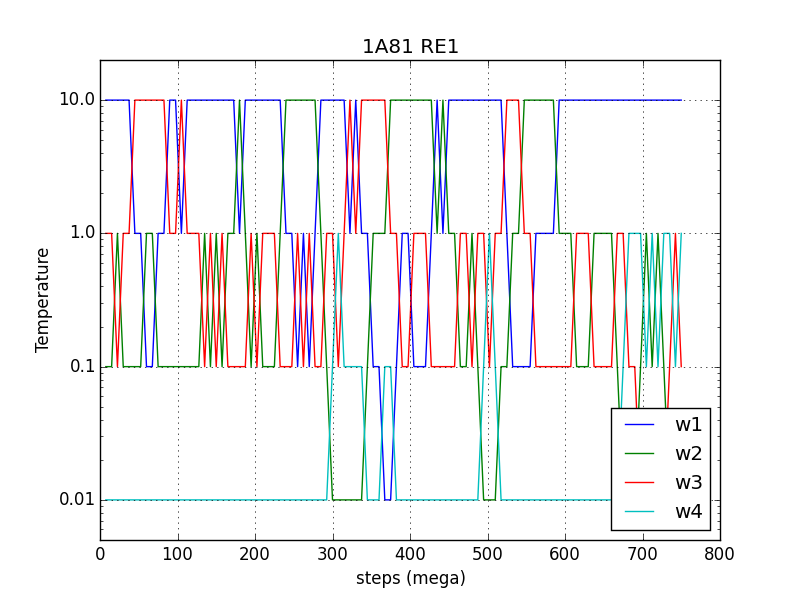
\includegraphics[width=8.45cm]{resultats/comparaisons/graphe/1A81-RE1-T_traj.png} &
       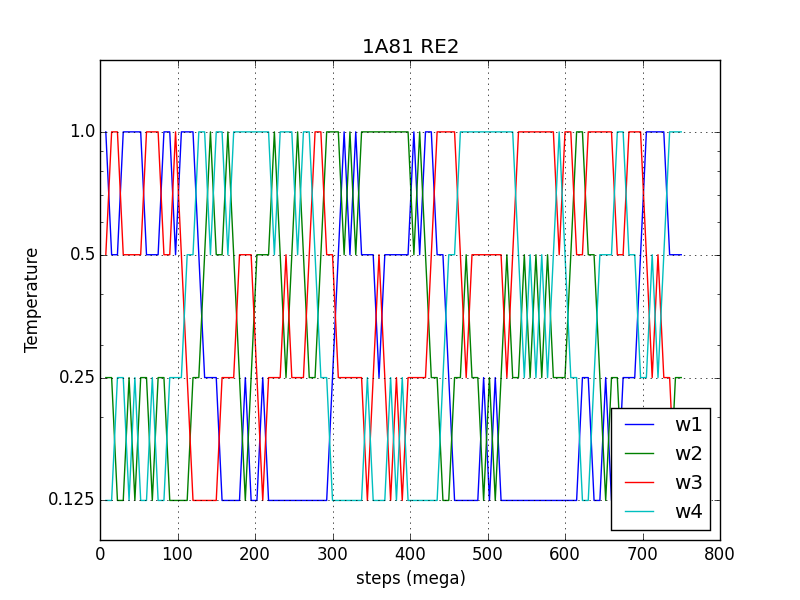
\includegraphics[width=8.45cm]{resultats/comparaisons/graphe/1A81-RE2-T_traj.png} \\
       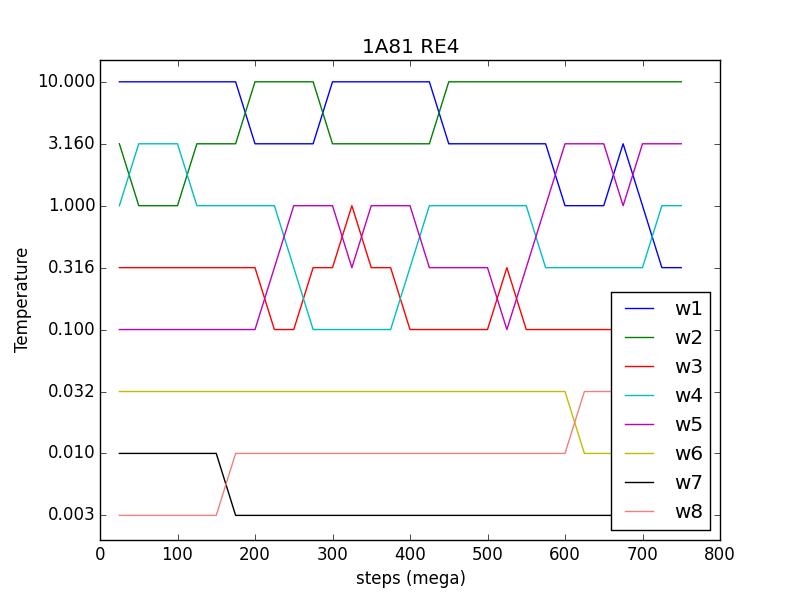
\includegraphics[width=8.45cm]{resultats/comparaisons/graphe/1A81-RE4-T_traj.png} &
       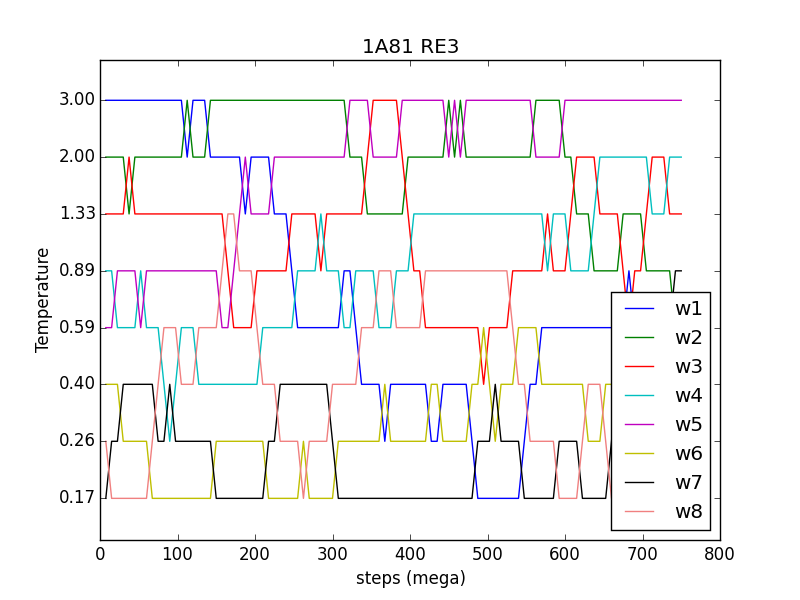
\includegraphics[width=8.45cm]{resultats/comparaisons/graphe/1A81-RE3-T_traj.png} \\
     \end{tabular}
     \caption{Variation de la température au court de la trajectoire de chaque marcheur (protocole RE1).}
     \label{TRAJ_T}
   \end{figure}

    \clearpage

   \begin{figure}[t]
     \centering
     \begin{tabular}{cc}
       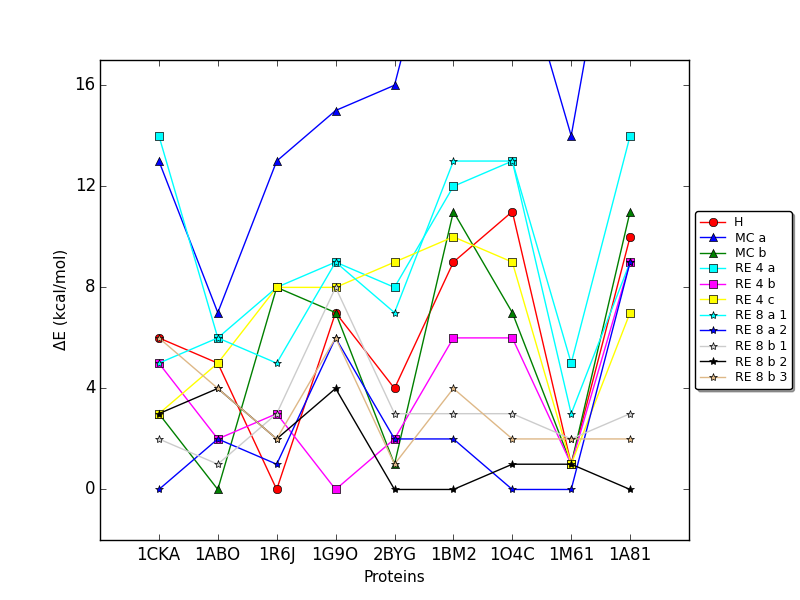
\includegraphics[width=18cm]{resultats/comparaisons/graphe/best_all.png} \\
     \end{tabular}
     \caption{Tous les protocoles.}
     \label{TRAJ_T}
   \end{figure}


    \clearpage


   \begin{figure}[t]
     \centering
     \begin{tabular}{cc}
       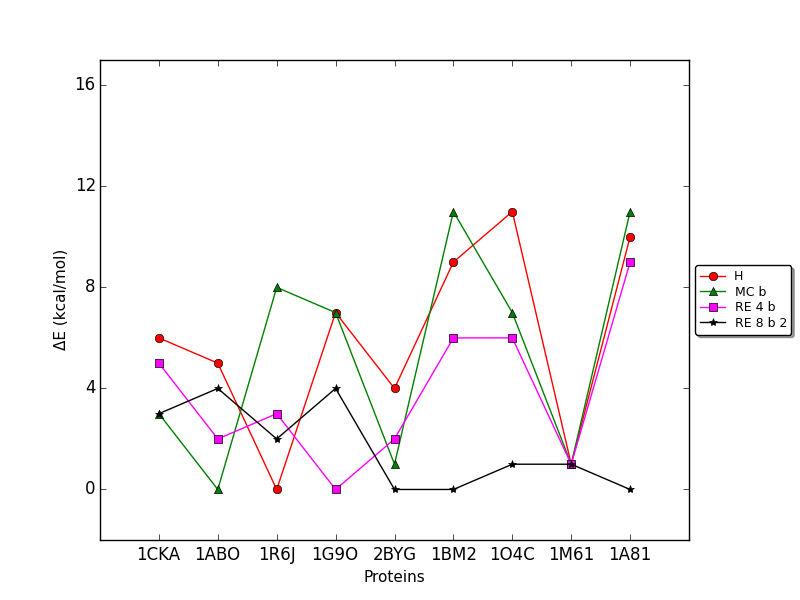
\includegraphics[width=8cm]{resultats/comparaisons/graphe/best_by_cat.png} &
       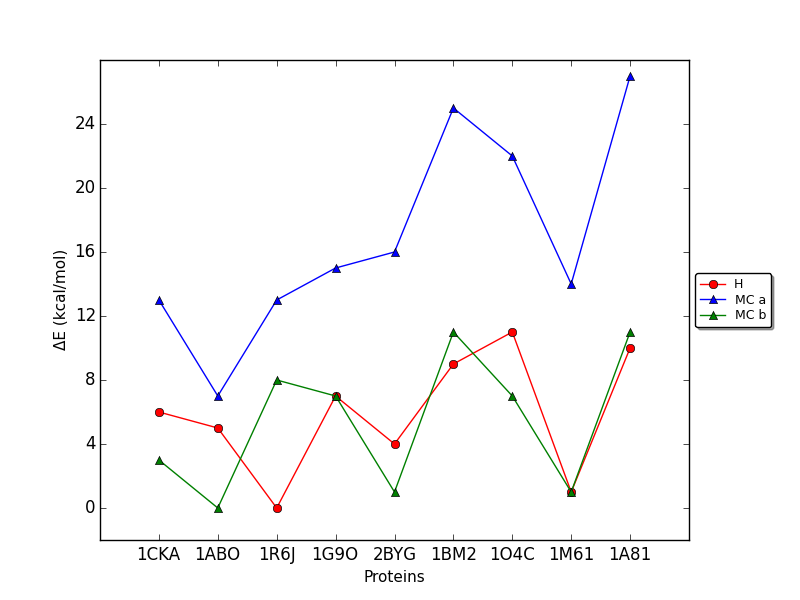
\includegraphics[width=8cm]{resultats/comparaisons/graphe/best_MC+H.png} \\
       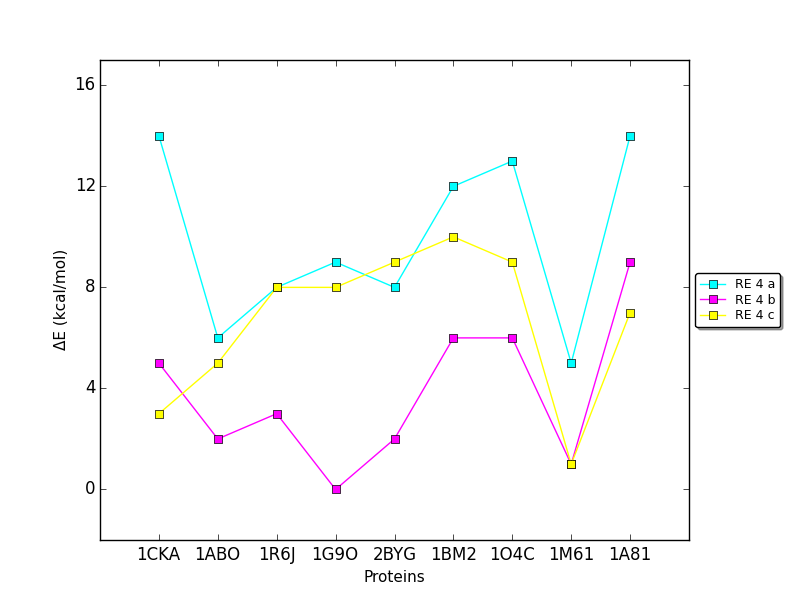
\includegraphics[width=8cm]{resultats/comparaisons/graphe/best_RE4.png} &
       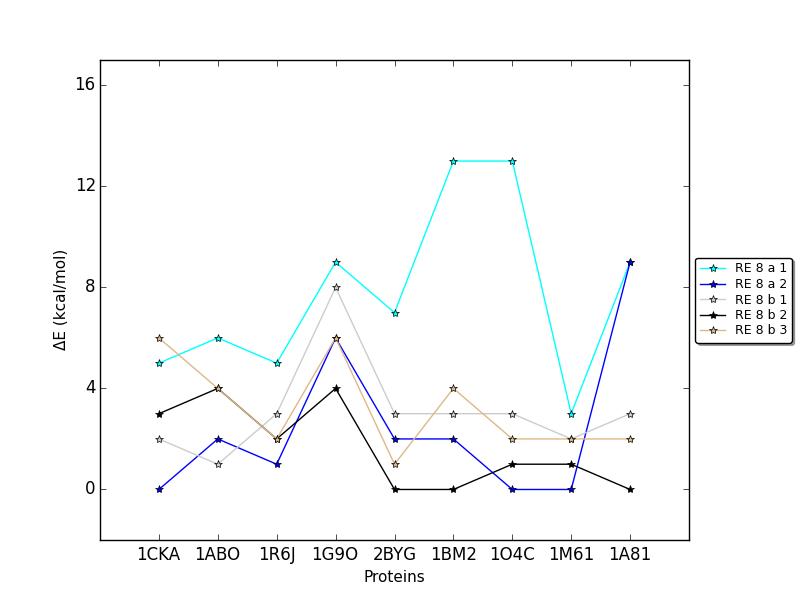
\includegraphics[width=8cm]{resultats/comparaisons/graphe/best_RE8.png} \\
     \end{tabular}
     \caption{Variation de la température au court de la trajectoire de chaque marcheur (protocole RE1).}
     \label{TRAJ_T}
   \end{figure}


    \clearpage

   \subsection{Avec des résidus gelés}
 
   \subsubsection{Séquence native}

 
    \begin{table}[h]
      \centering

      \begin{tabular}{|c|c|c|c|c|c|c|}

        \hline
        Protéine & GMEC & H- & MC0 & MC4- \\
        \hline
        1A81 & -585.1365 & 0 & -0.2547 & 0 \\
        1ABO & -320.1798 & 0 & 0 & 0 \\
        1BM2 & -553.5532 & 0 & -0.0564 & -0.0121 \\
        1CKA & -319.2787 & 0 & 0 & 0 \\
        1G9O & -481.1175 & 0 & -0.1394 & 0 \\
        1M61 & -555.9140 & 0 & 0 & 0 \\
        1O4C & -591.2115 & 0 & 0 & -0.1250 \\
        1R6J & -454.9340 & 0 & 0 & 0 \\
        2BYG & -507.0165 & 0 & 0 & 0 \\        
        \hline


      \end{tabular}      
      \caption{L’énergie du GMEC et la différence avec les autres protocoles.Tous les résidus sont gelés}
      \label{tab_best_ener_no_active}      
    \end{table}


   \subsubsection{Une position active}


    \begin{table}[h]
      \centering

      \begin{tabular}{|c|c|c|}


        \hline
        Position & GMEC & MC4- \\
        \hline
        14 & -584.4693 & -0.0405 \\
        39 & -584.7378 & -0.0111 \\
        55 & -584.0477 & -0.0012 \\
        60 & -583.7763 & -0.0140 \\
        66 & -592.3835 & -0.0347 \\
        70 & -583.8950 & -0.0348 \\
        71 & -588.5916 & -0.0247 \\
        76 & -583.3815 & -0.0248 \\
        79 & -582.8485 & -0.0406 \\
        86 & -584.1412 & -0.0248 \\
        101 & -583.8406 & -0.0248 \\
        105 & -583.0197 & -0.0248 \\
        107 & -582.2241 & -0.0248 \\

        \hline


      \end{tabular}      
      \caption{Liste des échecs pour 1A81}
      \label{tab_best_ener_no_active}      
    \end{table}


    \begin{table}[h]
      \centering

      \begin{tabular}{|c|c|c|}


        \hline
        Position & GMEC & MC4- \\
        \hline
        2 & -553.3134 & -0.0040 \\
        3 & -553.5532 & -0.0121 \\
        5 & -553.0932 & -0.0179 \\
        6 & -553.5532 & -0.0121 \\
        8 & -556.1917 & -0.0148 \\
        10 & -551.4990 & -0.0149 \\
        11 & -551.8859 & -0.0149 \\
        12 & -550.8152 & -0.0148 \\
        13 & -553.4829 & -0.0451 \\
        14 & -553.5532 & -0.0121 \\
        15 & -553.5532 & -0.0121 \\
        17 & -553.5532 & -0.0121 \\
        18 & -553.0880 & -0.0121 \\
        19 & -553.5532 & -0.0270 \\
        20 & -553.0003 & -0.0121 \\
        21 & -553.5532 & -0.0121 \\
        22 & -553.1769 & -0.0121 \\
        29 & -553.5532 & -0.0121 \\
        34 & -553.5532 & -0.0270 \\
        36 & -555.3358 & -0.0317 \\
        37 & -553.5532 & -0.0121 \\
        41 & -553.5076 & -0.0121 \\
        46 & -552.9056 & -0.0149 \\
        49 & -553.5532 & -0.0121 \\
        51 & -553.5532 & -0.0179 \\
        55 & -551.8384 & -0.0121 \\
        56 & -553.5532 & -0.0121 \\
        57 & -561.0695 & -0.0121 \\
        58 & -553.5532 & -0.0121 \\
        62 & -553.5532 & -0.0121 \\
        65 & -553.5532 & -0.0121 \\
        66 & -551.2026 & -0.0179 \\
        68 & -552.6182 & -0.0148 \\
        70 & -553.5532 & -0.0121 \\
        72 & -552.2724 & -0.0121 \\
        73 & -553.5532 & -0.0121 \\
        75 & -553.5532 & -0.0179 \\
        77 & -553.0234 & -0.0466 \\
        80 & -553.5532 & -0.0121 \\
        81 & -553.5532 & -0.0121 \\
        82 & -548.0641 & -0.0121 \\
        83 & -553.5532 & -0.0121 \\
        85 & -550.1884 & -0.0122 \\
        86 & -552.7375 & -0.0148 \\
        87 & -550.6139 & -0.0121 \\
        90 & -552.8601 & -0.0009 \\
        91 & -553.5532 & -0.0121 \\
        92 & -553.5532 & -0.0121 \\
        93 & -553.2772 & -0.0148 \\
        94 & -553.3207 & -0.0251 \\
        96 & -553.5532 & -0.0121 \\
        \hline


      \end{tabular}      
      \caption{Liste des échecs pour 1BM2}
      \label{tab_best_ener_no_active}      
    \end{table}




    \begin{table}[h]
      \centering

      \begin{tabular}{|c|c|c|}


        \hline
        Position & GMEC & MC4- \\
        \hline
        17 & -316.1693 & -0.0109 \\

\hline
      \end{tabular}      
      \caption{Liste des échecs pour 1CKA}
      \label{tab_echec_1CKA_1}      
    \end{table}

    \begin{table}[h]
      \centering

      \begin{tabular}{|c|c|c|}

        \hline
        \hline
        Position & GMEC & MC4 \\
        \hline
        58 & -561.9469 & -0.0138 \\
        
        \hline

      \end{tabular}      
      \caption{Liste des échecs pour 1M61}
      \label{tab_echec1M61__1}      
    \end{table}
    

    \begin{table}[h]
      \centering
      
      \begin{tabular}{|c|c|c|}
        



        \hline
        Position & GMEC & MC4- \\
        \hline
        1 & -591.2115 & -0.1380 \\
        2 & -591.2115 & -0.1250 \\
        3 & -591.2115 & -0.1250 \\
        4 & -590.7216 & -0.0319 \\
        5 & -590.5458 & -0.1071 \\
        6 & -591.2115 & -0.1521 \\
        7 & -590.7923 & -0.1429 \\
        8 & -591.2115 & -0.1250 \\
        9 & -591.2115 & -0.1728 \\
        10 & -591.2115 & -0.2572 \\
        11 & -589.9443 & -0.2489 \\
        12 & -591.1022 & -0.1137 \\
        13 & -589.9867 & -0.0535 \\
        14 & -591.2115 & -0.1250 \\
        15 & -589.4899 & -0.0436 \\
        16 & -591.2115 & -0.1521 \\
        17 & -590.4460 & -0.0557 \\
        18 & -589.0053 & -0.1366 \\
        19 & -590.7580 & -0.0348 \\
        20 & -591.2115 & -0.1250 \\
        21 & -591.2115 & -0.1600 \\
        22 & -591.2115 & -0.1250 \\
        23 & -590.5249 & -0.1530 \\
        24 & -590.7262 & -0.0630 \\
        25 & -591.2115 & -0.1250 \\
        26 & -591.2115 & -0.1250 \\
        27 & -590.8058 & -0.1194 \\
        28 & -591.2115 & -0.1250 \\
        29 & -591.2115 & -0.1571 \\
        30 & -590.5207 & -0.0221 \\
        31 & -590.5507 & -0.0530 \\
        32 & -591.2115 & -0.1571 \\
        33 & -591.2115 & -0.1234 \\
        34 & -590.7486 & -0.1258 \\
        35 & -591.2115 & -0.0378 \\
        36 & -589.1510 & -0.0974 \\
        37 & -591.0133 & -0.0941 \\
        38 & -589.2126 & -0.2743 \\
        39 & -589.0387 & -0.1890 \\
        40 & -590.8793 & -0.0883 \\
        41 & -589.4209 & -0.0409 \\
        42 & -591.2115 & -0.1250 \\
        43 & -587.9420 & -0.1315 \\
        44 & -589.8470 & -0.0595 \\
        45 & -591.2115 & -0.1712 \\
        46 & -588.8346 & -0.2668 \\
        47 & -589.9117 & -0.2773 \\
        48 & -588.6520 & -0.2625 \\
        49 & -591.2115 & -0.2120 \\
        50 & -590.6561 & -0.0807 \\
        51 & -591.1249 & -0.2986 \\
        52 & -589.7127 & -0.2734 \\
        53 & -590.7224 & -0.3012 \\
        54 & -590.8735 & -0.3615 \\
        55 & -588.6242 & -0.2007 \\
        56 & -591.2115 & -0.2120 \\
        57 & -591.2115 & -0.1250 \\
        58 & -590.6832 & -0.0743 \\
        59 & -591.2115 & -0.0378 \\
        60 & -591.1842 & -0.1082 \\
        61 & -590.6996 & -0.1272 \\
        62 & -595.8620 & -0.0899  \\
        63 & -591.2115 & -0.0974 \\
        64 & -588.8836 & -0.1014 \\
        65 & -591.2115 & -0.1571 \\
        66 & -590.1420 & -0.1533 \\
        67 & -587.5415 & -0.0433 \\
        68 & -590.1771 & -0.1541 \\
        69 & -591.2115 & -0.1250 \\
        70 & -590.4684 & -0.1066 \\
        71 & -591.2115 & -0.1250 \\
        72 & -591.2115 & -0.1311 \\
        73 & -591.2115 & -0.1250 \\
        74 & -588.7096 & -0.1169 \\
        75 & -590.2437 & -0.0505 \\
        76 & -591.2115 & -0.1521 \\
        78 & -587.6940 & -0.0821 \\
        79 & -589.9770 & -0.1380 \\
        80 & -591.1165 & -0.0661 \\
        81 & -590.2528 & -0.1229 \\
        82 & -589.8459 & -0.0724 \\
        83 & -590.2079 & -0.0513 \\
        84 & -591.2095 & -0.0433 \\
        85 & -590.8011 & -0.1154 \\
        87 & -590.7787 & -0.0744 \\
        88 & -590.2860 & -0.0857 \\
        89 & -591.2115 & -0.1250 \\
        90 & -590.2493 & -0.1084 \\
        91 & -589.5602 & -0.0694 \\
        92 & -589.3260 & -0.1838 \\
        93 & -590.4697 & -0.0188 \\
        94 & -587.4192 & -0.3392 \\
        95 & -590.0201 & -0.2937 \\
        96 & -590.6312 & -0.2723 \\
        97 & -595.0049 & -0.2864 \\
        98 & -590.0135 & -0.2013 \\
        99 & -589.7855 & -0.2932 \\
        100 & -591.2115 & -0.2120 \\
        101 & -591.2115 & -0.2120 \\
        102 & -591.2115 & -0.2572 \\
        103 & -595.4168 & -0.1277 \\
        104 & -589.9208 & -0.3581 \\
        
        \hline


      \end{tabular}      
      \caption{Liste des échecs pour 1O4C}
      \label{tab_echec1O4C__1}      
    \end{table}

    \begin{table}[h]
      \centering

      \begin{tabular}{|c|c|c|}


        \hline
        Position & GMEC & MC4- \\
        \hline
         4 & -453.4484 & -0.0155  \\
        20 & -452.6464 & -0.0114 \\
        32 & -454.9340 & -0.0092 \\
        68 & -454.4856 & -0.0060 \\
        73 & -454.7809 & -0.0155 \\
        77 & -454.1344 & -0.0155 \\
        79 & -453.4729 & -0.0155 \\
        
        \hline


      \end{tabular}      
      \caption{Liste des échecs pour 1R6J }
      \label{tab_echec1R6J__1}      
    \end{table}


    \begin{table}[h]
      \centering

      \begin{tabular}{|c|c|c|}

        \hline
        Position & GMEC & MC4- \\
        \hline
        1 & -505.2910 & -0.0132 \\
        3 & -506.7960 & -0.0254 \\
        4 & -505.5800 & -0.0023 \\
        5 & -506.8732 & -0.0948 \\
        49 & -505.5183 & -0.0135 \\
        59 & -507.0165 & -0.0100 \\
        85 & -506.6217 & -0.0101 \\
        88 & -505.2286 & -0.0097 \\
        95 & -506.3195 & -0.0131 \\

        \hline


      \end{tabular}      
      \caption{Liste des échecs pour 2BYG }
      \label{tab_echec2BYG__1}      
    \end{table}


   \subsubsection{ Cinq positions actives}


    \begin{table}[h]
      \centering

      \begin{tabular}{|c|c|c|c|c|}


        \hline
        \hline
        Protéine & GMEC & H & MC4 & RE3 \\
        \hline
        1A81 1 & -579.3989 & 0 & 0 &  \\
        1A81 2 & -575.2254 & 0 & 0 &  \\
        1A81 3 & -582.7452 & 0 & 0 &  \\
        1A81 4 & -569.9383 & 0 & -5.3443 & 0 \\
        1A81 5 & -591.8143 & 0 & 0 &  \\
        1ABO 1 & -315.4497 & 0 & 0 &  \\
        1ABO 2 & -316.6637 & 0 & 0 &  \\
        1ABO 3 & -307.4824 & 0 & 0 &  \\
        1ABO 4 & -313.7710 & 0 & 0 &  \\
        1ABO 5 & -313.5695 & 0 & 0 &  \\
        1BM2 1 & -548.2341 & 0 & 0 &  \\
        1BM2 2 & -554.8135 & 0 & 0 &  \\
        1BM2 3 & -557.8629 & 0 & 0 &  \\
        1BM2 4 & -544.9791 & 0 & 0 &  \\
        1BM2 5 & -550.2956 & 0 & -0.0121 &  \\
        1CKA 1 & -315.0859 & 0 & 0 &  \\
        1CKA 2 & -309.7692 & 0 & 0 &  \\
        1CKA 3 & -317.3820 & 0 & 0 &  \\
        1CKA 4 & -314.8550 & 0 & 0 &  \\
        1CKA 5 & -312.0405 & -0.0001 & -0.0001 &  \\
        1G9O 1 & -469.9540 & 0 & 0 &  \\
        1G9O 2 & -476.4094 & 0 & 0 &  \\
        1G9O 3 & -479.7190 & 0 & 0 &  \\
        1G9O 4 & -478.9513 & 0 & 0 &  \\
        1G9O 5 & -480.7260 & 0 & 0 &  \\
        1M61 1 & -557.6647 & 0 & 0 &  \\
        1M61 2 & -546.9587 & 0 & 0 &  \\
        1M61 3 & -553.0731 & 0 & 0 &  \\
        1M61 4 & -555.0885 & 0 & 0 &  \\
        1M61 5 & -554.6356 & 0 & 0 &  \\
        1O4C 1 & -584.4267 & 0 & -0.0655 &  \\
        1O4C 2 & -584.8989 & 0 & -0.1437 &  \\
        1O4C 3 & -588.4971 & 0 & -0.1164 &  \\
        1O4C 4 & -587.7129 & 0 & -0.1400 &  \\
        1O4C 5 & -587.6514 & 0 & -0.1168 &  \\
        1R6J 1 & -444.5018 & 0 & 0 &  \\
        1R6J 2 & -449.3043 & 0 & -0.9421 & 0 \\
        1R6J 3 & -453.1139 & 0 & 0 &  \\
        1R6J 4 & -453.1139 & 0 & 0 &  \\
        1R6J 5 & -454.9340 & 0 & 0 &  \\
        2BYG 1 & -500.7946 & 0 & -0.0150 &  \\
        2BYG 2 & -506.2319 & 0 & 0 &  \\
        2BYG 3 & -506.8744 & 0 & -0.0131 &  \\
        2BYG 4 & -504.5135 & 0 & 0 &  \\
        2BYG 5 & -506.0052 & 0 & 0 &  \\

        \hline




 \end{tabular}      
 \caption{Résultats 5 position actives}
 \label{tab_echec2BYG__1}      
\end{table}


   \subsubsection{ Dix positions actives}


    \begin{table}[h]
      \centering

      \begin{tabular}{|c|c|c|c|c|}


        \hline
        Protéine & GMEC & H & MC4 & RE32 \\
        \hline
        1A81 1 & -583.9354 & 0 & 0 & \\
        1A81 2 & -581.7802 & 0 & 0 & \\
        1A81 3 & -587.4392 & -0.0001 & -0.1595 & \\
        1A81 4 & -589.1322 & 0 & -0.0317 & \\
        1A81 5 & -578.2558 & 0 & -0.0563 & \\
        1ABO 1 & -309.1670 & -0.0675 & -0.9054 & \\
        1ABO 2 & -308.8387 & 0 & 0 & \\
        1ABO 3 & -303.8520 & 0 & 0 & \\
        1ABO 4 & -310.0087 & 0 & -0.0128 & \\
        1ABO 5 & -301.6727 & 0 & 0 & \\
        1BM2 1 & -549.8638 & 0 & -0.0950 & \\
        1BM2 2 & -541.5944 & 0 & 0 & \\
        1BM2 3 & -543.7434 & 0 & 0 & \\
        1BM2 4 & -549.0453 & 0 & 0 & \\
        1BM2 5 & -544.1447 & 0 & -0.1082 & \\
        1CKA 1 & -305.8477 & 0 & 0 & \\
        1CKA 2 & -309.9886 & 0 & 0 & \\
        1CKA 3 & -304.6618 & 0 & 0 & \\
        1CKA 4 & -302.4894 & 0 & 0 & \\
        1CKA 5 & -299.2329 & -0.2859 & -3.2525 & 0 \\
        1G9O 1 & -466.6764 & 0 & 0 & \\
        1G9O 2 & -478.8797 & 0 & 0 & \\
        1G9O 3 & -477.2503 & -0.1366 & 0 & \\
        1G9O 4 & -470.6458 & 0 & 0 & \\
        1G9O 5 & -464.8659 & 0 & -3.9599 & \\
        1M61 1 & -550.0699 & 0 & -0.0776 & \\
        1M61 2 & -538.6026 & -3.5105 & -4.5062 & 0.3215 \\
        1M61 3 & -552.2673 & 0 & 0 & \\
        1M61 4 & -550.0553 & 0 & 0 & \\
        1M61 5 & -553.6559 & 0 & -0.0432 & \\
        1O4C 1 & -587.4665 & 0 & -0.1121 & \\
        1O4C 2 & -585.8545 & 0 & -0.1046 & \\
        1O4C 3 & -580.3505 & 0 & -0.1519 & \\
        1O4C 4 & -587.1548 & 0 & -0.1545 & \\
        1O4C 5 & -590.2650 & 0 & -0.1753 & \\
        1R6J 1 & -448.8351 & 0 & -2.4022 & -2.3986 \\
        1R6J 2 & -448.4631 & 0 & -1.0398 & \\
        1R6J 3 & -450.3950 & 0 & -0.0106 & \\
        1R6J 4 & -451.7211 & 0 & 0 & \\
        1R6J 5 & -450.9943 & 0 & -0.0162 & \\
        2BYG 1 & no & -505.6397 & -0.0337 & \\
        2BYG 2 & -504.7389 & 0 & 0 & \\
        2BYG 3 & -504.3048 & 0 & -0.0833 & \\
        2BYG 4 & -504.3466 & 0 & -0.2149 & \\
        2BYG 5 & -491.6095 & 0 & 0 & \\
        
        \hline


 \end{tabular}      
 \caption{Résultats 10 positions actives }
 \label{tab_echec2BYG__1}      
\end{table}


   \subsubsection{ Vingt et trente positions actives}



    \begin{table}[h]
      \centering

      \begin{tabular}{|c|c|c|c|c|c|c|c|c|}


        \hline
        \multicolumn{5}{|c|}{10 positions actives}  & \multicolumn{4}{|c|}{20 positions actives} \\
        \hline
        Protéine & GMEC & H & MC & RE & GMEC & H & MC & RE \\
        \hline
        1A81 1 & -583.9354 & 0 & 0 & & -566.9106 & 0 & -0.3275 & -.3851 \\             
        1A81 2 & -581.7802 & 0 & 0 & & -564.6618 & -0.1705 & -2.4355 & -1.0069 \\    
        1A81 3 & -587.4392 & -0.0001 & -0.1595 & & -572.9780 & 0 & -0.4640 & -.6186 \\       
        1A81 4 & -589.1322 & 0 & -0.0317 & & -570.3480 & -0.3568 & -0.5128 & -.6991 \\     
        1A81 5 & -578.2558 & 0 & -0.0563 & & -571.2480 & -0.7658 & -0.5088 & -.6991 \\     
        1ABO 1 & -309.1670 & -0.0675 & -0.9054 & & -299.6592 & -0.1205 & -1.1159 & -0.2153 \\    
        1ABO 2 & -308.8387 & 0 & 0 & & no & -298.3854 & 0 & 0 \\ 
        1ABO 3 & -303.8520 & 0 & 0 & & no & -298.3854 & 0 & 0 \\            
        1ABO 4 & -310.0087 & 0 & -0.0128 & & no & -297.8545 & -0.0076 & 0 \\          
        1ABO 5 & -301.6727 & 0 & 0 & & no & -297.8009 & -0.9483 & -.9483 \\       
        1BM2 1 & -549.8638 & 0 & -0.0950 & &   -526.0936 & 0 & -0.0619 & -.1584 \\        
        1BM2 2 & -541.5944 & 0 & 0 & & no & -525.3588 & -0.0725 & -.0143 \\       
        1BM2 3 & -543.7434 & 0 & 0 & & -534.3860 & -0.0230 & -0.4763 & -.2898 \\     
        1BM2 4 & -549.0453 & 0 & 0 & & no & -526.8307 & -2.5883 & -0.0789 \\       
        1BM2 5 & -544.1447 & 0 & -0.1082 & & -535.3334 & -0.2396 & -0.3746 & -.3746 \\     
        1CKA 1 & -305.8477 & 0 & 0 & & -295.6311 & 0 & 0 & 0\\  
        1CKA 2 & -309.9886 & 0 & 0 & & -295.8571 & 0 & 0 & 0 \\ 
        1CKA 3 & -304.6618 & 0 & 0 & & -293.8687 & 0 & 0 & 0 \\ 
        1CKA 4 & -302.4894 & 0 & 0 & & no & -293.8687 & 0 & 0 \\ 
        1CKA 5 & -299.2329 & -0.2859 & -3.2525 & 0 & no & -293.4203 & 0 & 0 \\ 
        1G9O 1 & -466.6764 & 0 & 0 & & no & -451.4604 & -1.2525 & -1.2525 \\       
        1G9O 2 & -478.8797 & 0 & 0 & & no & -453.2355 & -0.2487 & -.1915 \\       
        1G9O 3 & -477.2503 & -0.1366 & 0 & & no & -453.2474 & -0.2177 & -.1915 \\       
        1G9O 4 & -470.6458 & 0 & 0 & & no & -456.3751 & -0.2275 & -.1455 \\       
        1G9O 5 & -464.8659 & 0 & -3.9599 & & no & -456.7331 & -0.1455 & -.1455 \\       
        1M61 1 & -550.0699 & 0 & -0.0776 & & -528.0700 & 0 & 0 & 0 \\ 
        1M61 2 & -538.6026 & -3.5105 & -4.5062 & 0.3215 & -528.7653 & 0 & 0 & 0 \\ 
        1M61 3 & -552.2673 & 0 & 0 & & -530.0684 & 0 & 0 & 0 \\ 
        1M61 4 & -550.0553 & 0 & 0 & & -534.5248 & 0 & 0 & 0 \\ 
        1M61 5 & -553.6559 & 0 & -0.0432 & & -548.0096 & 0 & -0.2521 & -0.1345 \\          
        1O4C 1 & -587.4665 & 0 & -0.1121 & & no & -.2878 & -.0103 & -574.0634 \\        
        1O4C 2 & -585.8545 & 0 & -0.1046 & & no & -574.8584 & -0.1963 & -.3175 \\       
        1O4C 3 & -580.3505 & 0 & -0.1519 & & -573.6314 & 0 & -0.3461 & -.0997 \\        
        1O4C 4 & -587.1548 & 0 & -0.1545 & & -575.8667 & 0 & -0.3640 & -.1382 \\        
        1O4C 5 & -590.2650 & 0 & -0.1753 & & no & -573.3479 & -0.1141 & -.2206 \\       
        1R6J 1 & -448.8351 & 0 & -2.4022 & -0.3986 & -440.7417 & 0 & -0.2604 & -.2002 \\        
        1R6J 2 & -448.4631 & 0 & -1.0398 & & -437.2537 & 0 & -0.0071 & -.0183 \\        
        1R6J 3 & -450.3950 & 0 & -0.0106 & & -439.4335 & 0 & -0.0537 & -.0732 \\        
        1R6J 4 & -451.7211 & 0 & 0 & & -439.9135 & 0 & -0.0537 & -.0732 \\        
        1R6J 5 & -450.9943 & 0 & -0.0162 & & -438.0222 & 0 & -0.0735 & -.0244 \\        
        2BYG 1 & no & -505.6397 & -0.0337 & & -496.2991 & 0 & -3.1878 & -.0257 \\        
        2BYG 2 & -504.7389 & 0 & 0 & & -494.8723 & 0 & -0.0524 & -.0826 \\        
        2BYG 3 & -504.3048 & 0 & -0.0833 & & -494.8723 & 0 & -1.3564 & -.0826 \\        
        2BYG 4 & -504.3466 & 0 & -0.2149 & & -495.9213 & 0 & -0.1968 & -.6022 \\        
        2BYG 5 & -491.6095 & 0 & 0 & & no & -497.5123 & -0.0933 & -.0386 \\       
    
    \hline


 \end{tabular}      
 \label{tab_echec_10_20}      
\end{table}





   \subsection{ Etude au voisinnage de GMECs}


    \begin{table}[h]
      \centering

      \begin{tabular}{|c|c|c|c|c|}

        Protéine & nb seq (GMEC + 1) & rang H &rang MC & rang RE \\
        \hline

        1CKA 3 &  67668 & 1 & 1 & \\
        1CKA 4 &  4647 & 1 & 1 & \\
        1CKA 5 &  255 &  10 & 182638 & 1 \\
        1G9O 3 &  435881 & 24 & 1 \\
        1G9O 4 &  354476 & 1 & 1 \\
        1G9O 5 &  61 & 1 & 897112 & 1 \\
        1M61 2 &  261467 &  & \\
        1M61 3 &  11199152 & 1 & 1 &\\
        1M61 4 &  16417603  & 1 & 1 & \\
        \hline


 \end{tabular}      
 \caption{Résultats 30 positions actives }
 \label{tab_echec2BYG__1}      
\end{table}


    \clearpage
    
    \begin{figure}[h]
      \centering
      \begin{tabular}{c} 
        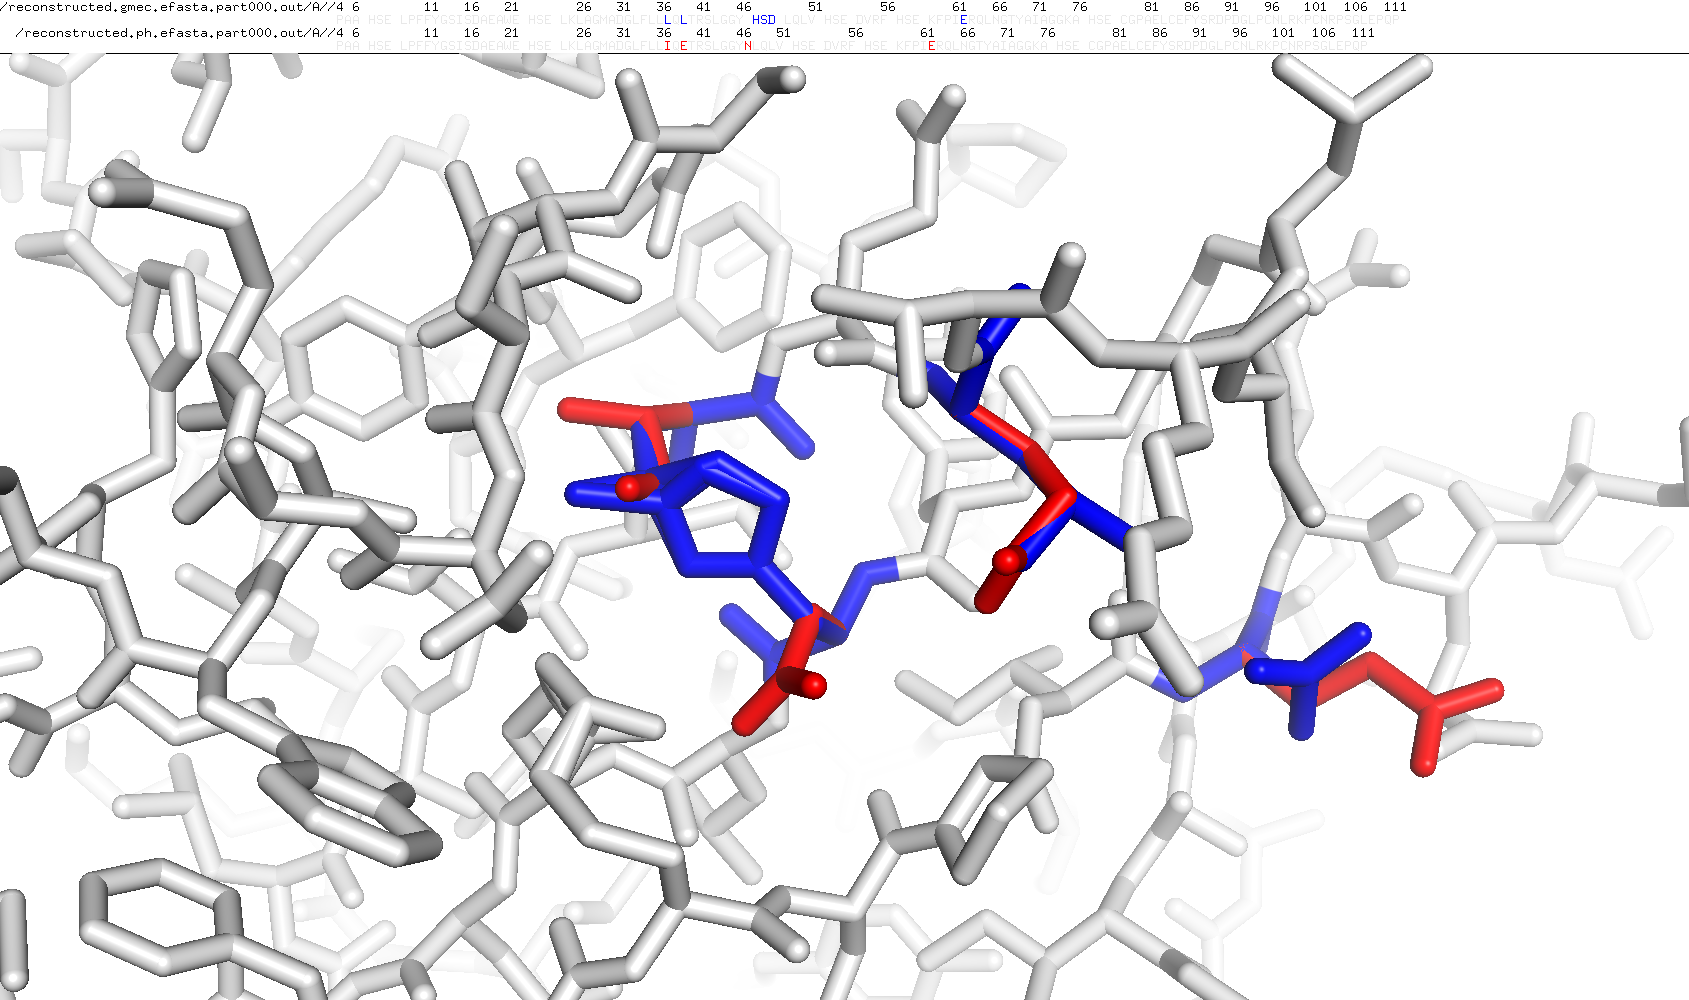
\includegraphics[width=14cm]{resultats/comparaisons/image/1M61_2_gmec_vs_ph.png} 
      \end{tabular}
      
      \caption{test: 1M61 2, GMEC vs H}
      \label{temps_CPU}
    \end{figure}
    
    
    
    \begin{figure}[h]
      \centering
      \begin{tabular}{c} 
        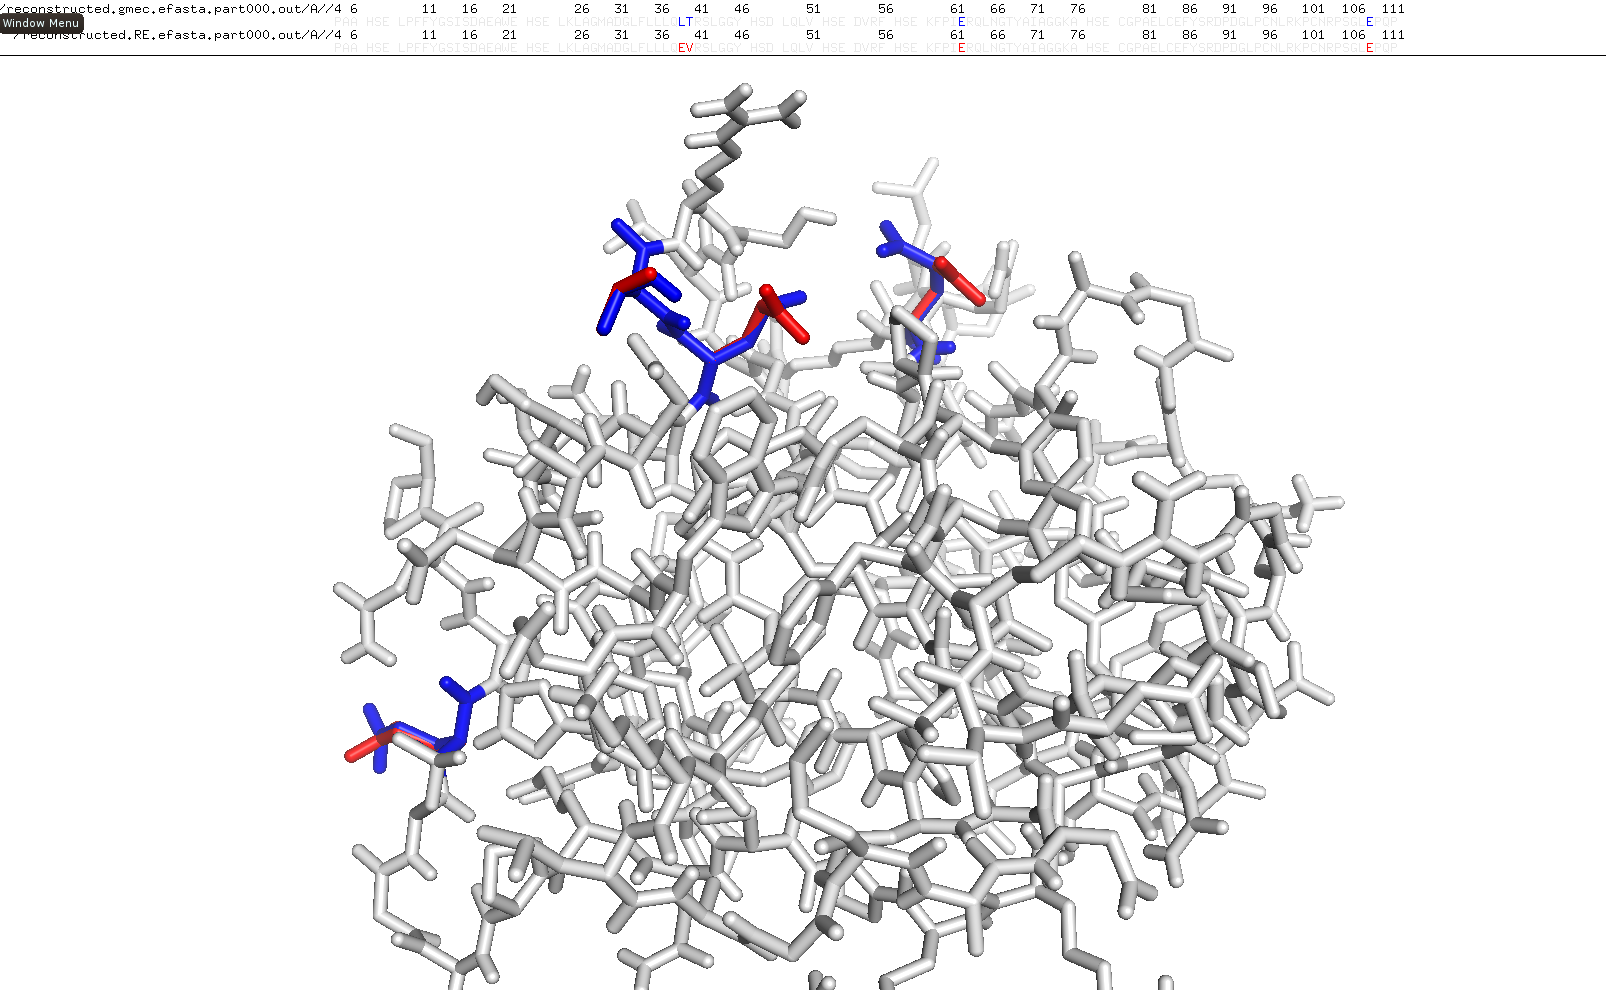
\includegraphics[width=14cm]{resultats/comparaisons/image/1M61_2_gmec_vs_RE.png} 
      \end{tabular}
      
      \caption{test: 1M61 2, GMEC vs RE}
      \label{temps_CPU}
    \end{figure}
    
    
    

    \begin{figure}[h]
      \centering
      \begin{tabular}{c} 
        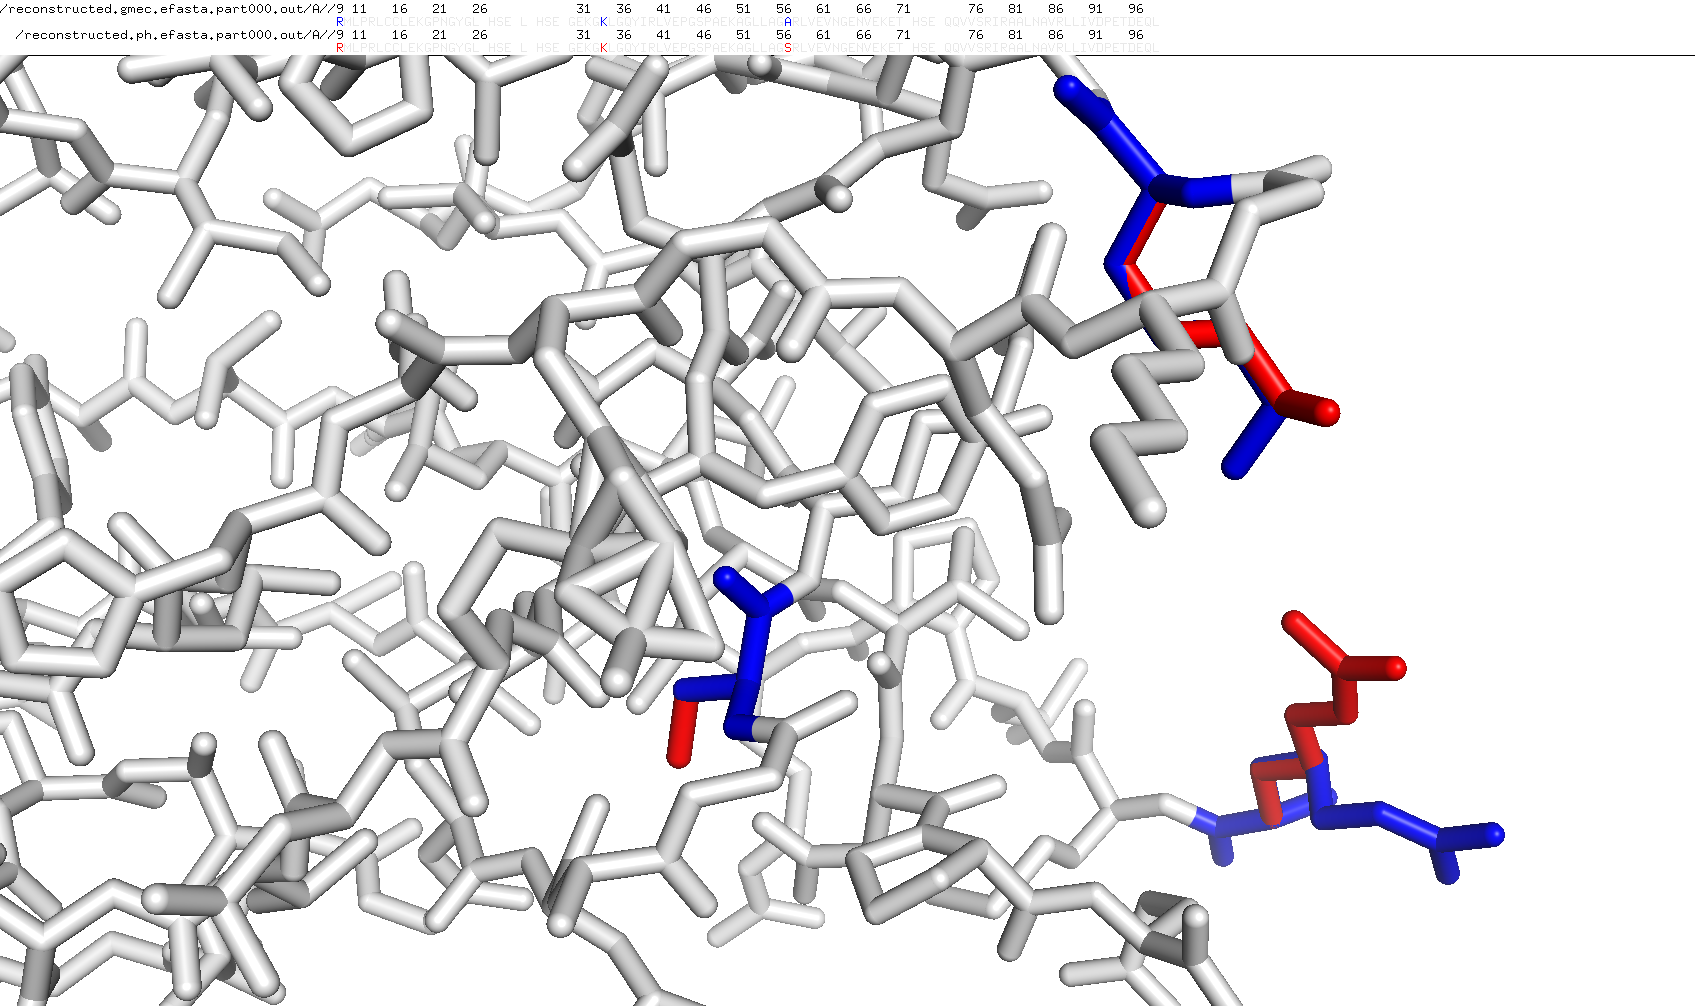
\includegraphics[width=14cm]{resultats/comparaisons/image/1G9O_3_gmec_vs_ph.png} 
      \end{tabular}
      
      \caption{test: 1G9O 3, GMEC vs H}
      \label{temps_CPU}
    \end{figure}
    
    
    \begin{figure}[h]
      \centering
      \begin{tabular}{c} 
        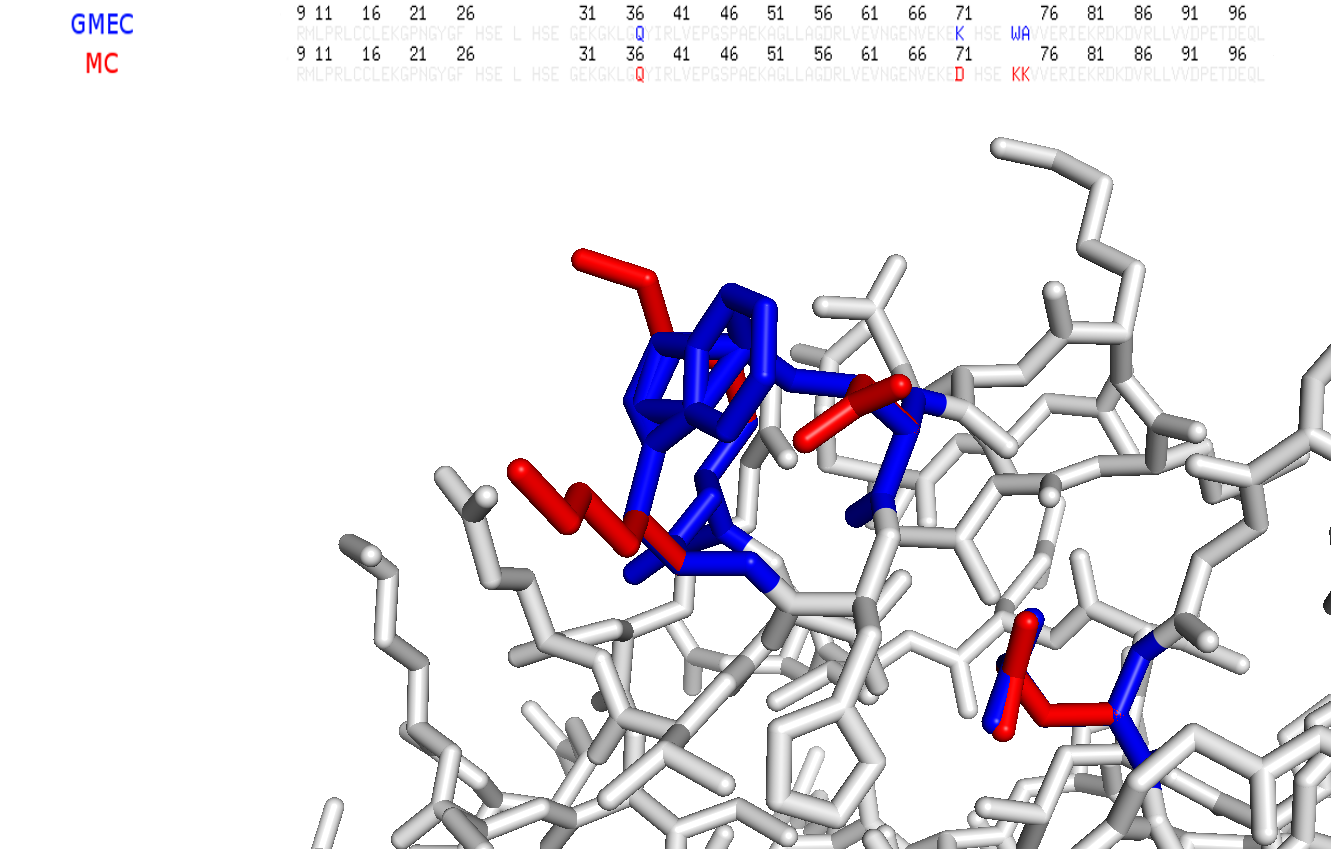
\includegraphics[width=14cm]{resultats/comparaisons/image/1G9O_5_gmec_vs_MC.png} 
      \end{tabular}
      
      \caption{test: 1G9O 5, GMEC vs MC}
      \label{temps_CPU}
    \end{figure}
    
    \begin{figure}[h]
      \centering
      \begin{tabular}{c} 
        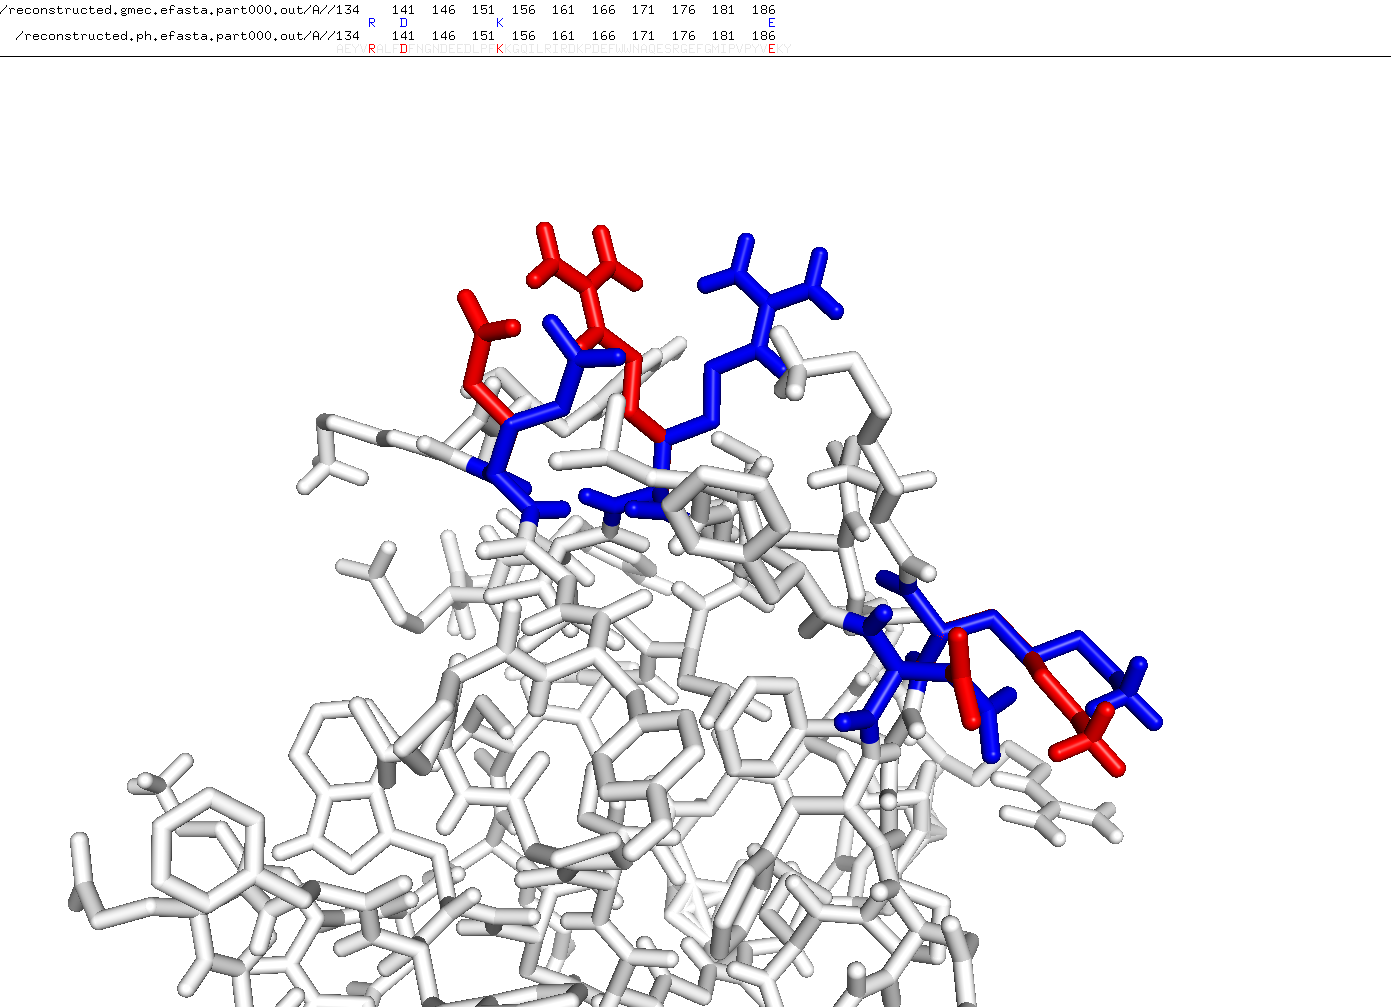
\includegraphics[width=14cm]{resultats/comparaisons/image/1CKA_5_gmec_vs_ph.png} 
      \end{tabular}
      
      \caption{test: 1CKA 5, GMEC vs H}
      \label{temps_CPU}
    \end{figure}
    
    

    \begin{figure}[h]
      \centering
      \begin{tabular}{c} 
        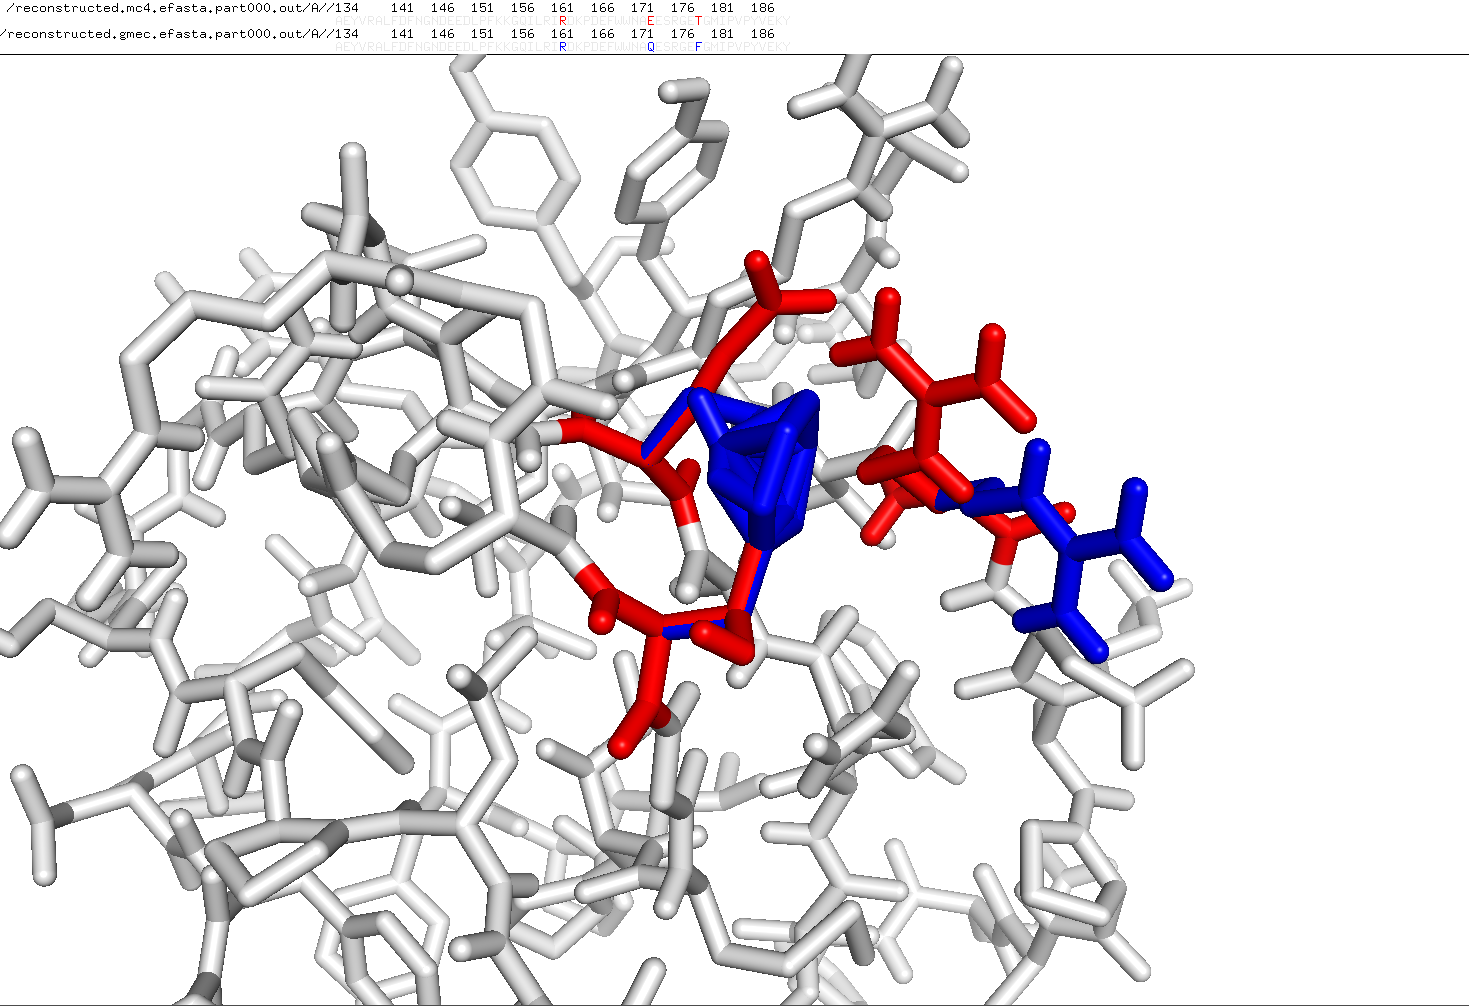
\includegraphics[width=14cm]{resultats/comparaisons/image/1CKA_5_gmec_vs_MC.png} 
      \end{tabular}
      
      \caption{test: 1CKA 5, GMEC vs MC}
      \label{temps_CPU}
    \end{figure}
    
    
    \clearpage





   \subsection{ Résultats Superfamily}


    \begin{table}[h]
           \raggedleft

      \begin{tabular}{|c|c|c|c|c|c|}

        \hline
        Protein & Match/seq size & Superfamily Evalue & superfamily success & Family Evalue & family success\\
        \hline
        1A81 & no & & & & \\
        1ABO & 51/58 & 4.4e-4 & 100\% & 2.8e-3 & 100\% \\
        1BM2 & 78/98 & 4.2e-5 & 100\% & 2.6e-3 & 100\% \\
        1CKA & 40/57 & 1.1e-5 & 100\% & 3.4e-3. & 100\% \\
        1G9O & 79/91 & 7.0e-7 & 100\% & 2.5e-3 & 100\%  \\
        1M61 & 97/109 & 7.2e-7 & 100\% & 2.6e-4 &  100\% \\
        1O4C & 95/104 & 2.1e-4 & 100\% & 4.5e-3 &  100\% \\
        1R6J & 74/82 & 9.8e-6 & 100\% & 4.6e-3 &  100\% \\
        2BYG & 59/97 & 1.4e-5 & 100\% & 7.1e-3 &  100\% \\

        \hline


 \end{tabular}      


 \label{tab_echec2BYG__1}       
\end{table}



    \clearpage


    \begin{table}[h]
      \centering

      \begin{tabular}{|c|c|c|c|c|}


        \hline
        Protein & GMEC & H & MC & RE \\
        \hline
        1CKA 3 & -304.6618 & 0 & 0 & \\
        1CKA 4 & -302.4894 & 0 & 0 & \\
        1CKA 5 & -299.2329 & -0.2859 & -3.2525 & 0 \\
        1G9O 3 & -477.2503 & -0.1366 & 0 & \\
        1G9O 4 & -470.6458 & 0 & 0 & \\
        1G9O 5 & -464.8659 & 0 & -3.9599 &  0 \\
        1M61 1 & -550.0699 & 0 & -0.0776 & \\
        1M61 2 & -538.6026 & -3.5105 & -4.5062 & 0.3215 \\
        1M61 5 & -553.6559 & 0 & -0.0432 & \\
        
        \hline


 \end{tabular}      
 \label{tab_1}      
\end{table}


    \begin{table}[h]
      \centering

      \begin{tabular}{|c|c|c|c|c|c|c|}


        \hline
        Protein & seq-rot nb gmec+1 & H rank  & MC rank  & seq nb gmec+1 & H mut nb & MC mut nb \\
        \hline
        1CKA 3 & 67669 & 1 & 1 & 227 & 0 & 0 \\
        1CKA 4 & 4649 & 1 & 1 & 498 & 0 & 0 \\
        1CKA 5 & 1388 & 78 & ? & 77 & 0 & 2 \\
        1G9O 3 & 354559 & 23 & 1 & 63 & 1 & 0 \\
        1G9O 4 & 22639 & 1 & 1 & 381 & 0 & 0 \\
        1G9O 5 & 8658395 & 1 & ? &  11 & 0 & 3 \\
        1M61 1 & 11199153 & ? & ? & 21 & 3 & 7 \\
        1M61 2 & 11199153 & 1 & 1 & 88 & 0 & 0 \\
        1M61 5 & 16417604 & 1 & 1 & 83 & 0 & 0 \\
        
        \hline


 \end{tabular}      
 \label{tab_2}      
\end{table}




    \clearpage

   \subsection{ Résultats Heuristic (protocoles longs)}


    \begin{table}[h]
      \centering

      \begin{tabular}{|c|c|c|c|c|}

        \hline
        Proteins & GMEC & H & H+ & H++ \\
        \hline
        1ABO 1 & -309.1670 & -0.0675 & -0.0675 & 0 \\
        1CKA 5 & -299.2329 & -0.2859 & -0.0640 & 0 \\
        1G9O 3 & -477.2503 & -0.1366 & 0 & 0 \\
        1M61 2 & -538.6026 & -3.5105 & -2.1673 & -0.0188 \\
        \hline


 \end{tabular}      
 \caption{Résultats pour 3 fois (resp 9 fois ) plus de cycles heuristiques protocole H+ (resp H++)}
 \label{tab_echec2BYG__1}       
\end{table}



    \clearpage

    \clearpage

   \subsection{densité en séquences }



    \begin{figure}[h]
      \centering
      \begin{tabular}{cc} 
        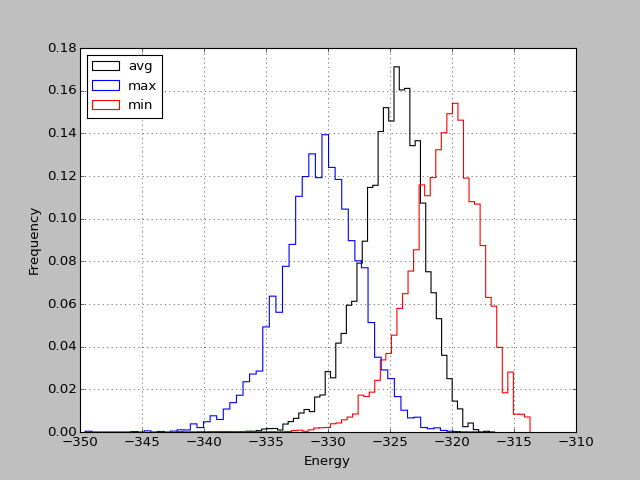
\includegraphics[width=10cm]{resultats/comparaisons/graphe/histo1_aa_Tambiante.png} &
      \end{tabular}
      
      \caption{.}
      \label{temps_CPU}
    \end{figure}


    \begin{figure}[h]
      \centering
      \begin{tabular}{cc} 
        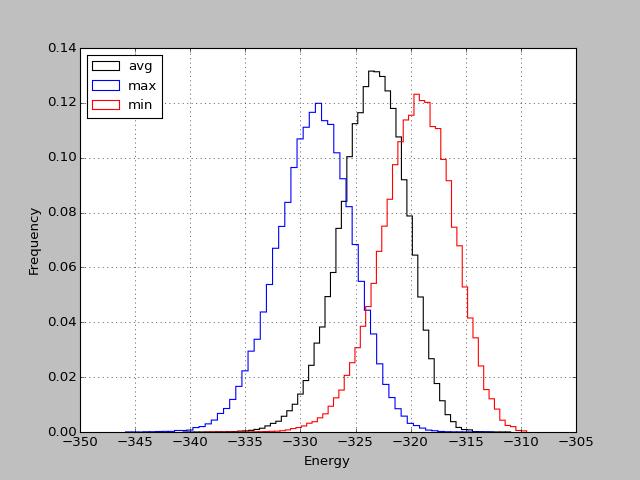
\includegraphics[width=10cm]{resultats/comparaisons/graphe/histo2_aa_Tambiante.png} &
      \end{tabular}
      
      \caption{.}
      \label{temps_CPU}
    \end{figure}

    \clearpage








% ---------------------
\clearplaindoublepage
\chapter{Titre d'une partie de r�sultats}
\label{chap:resultats2}

\section{Section}

XXX

\subsection{Subsection}

XXX

\subsubsection{Subsubsection}

XXX

\paragraph{Paragraph}

XXX

\subparagraph{Subparagraph}

R�f�rence � une table (Table~\ref{tab:label_table}).

\begin{table}[!htbp]
\centering

\caption{L�gende de la table}

\vspace{2ex}
\begin{tabular}{lcc}
\hline
Colonne1$^a$ & Colonne2$^b$ & Colonne3$^c$\\
\hline
X1 & X2 & X3\\
Y1 & Y2 & Y3\\
Z1 & Z2 & Z3\\
\hline
\end{tabular}

\bigskip

{\raggedright

$^a$ note1

$^b$ note2

$^c$ note3

}

\label{tab:label_table}
\end{table}

\clearplaindoublepage
\chapter*{Conclusion}
\label{chap:conc}
\addcontentsline{toc}{chapter}{Conclusion}
\markboth{Conclusion}{Conclusion}

XXX

\clearplaindoublepage
\appendix
\chapter{Titre d'une annexe}
\label{chap:annexe1}

XXX

\clearplaindoublepage
\chapter{1 Titre d'une annexe}
\label{chap:annexe2}

XXX

\clearplaindoublepage
\phantomsection
\addcontentsline{toc}{chapter}{Bibliographie}
\markboth{Bibliographie}{Bibliographie}
%\selectlanguage{english}
\renewcommand{\bibname}{Bibliographie}
\singlespacing
\bibliography{biblio}
\onehalfspacing
%\selectlanguage{frenchb}
\clearplaindoublepage

% Backmatter
\backmatter
\pagestyle{empty}
\addtolength{\oddsidemargin}{-0.5cm}
\addtolength{\evensidemargin}{+0.5cm}
\singlespacing
\selectlanguage{frenchb}

\pdfbookmark[0]{Resume}{resume}

\section*{Résumé}

{\large\bf\noindent Computational protein design: un outil pour l’ingénierie des protéines et la biologie synthétique}

\bigskip

Le CPD ou \og Computational protein design\fg est la recherche par modélisation moléculaire des séquences d’acides aminés compatibles avec une structure protéique ciblée. L’objectif est de concevoir une fonction nouvelle et/ou d’ajouter un nouveau comportement. Le CPD est en développement au sein de notre laboratoire depuis quelques années, avec le logiciel Proteus qui a plusieurs succès à son actif.

Au cours de cette Thèse, nous avons enrichi Proteus sur plusieurs points, avec notamment l’ajout d’une méthode d’exploration Monte Carlo avec échange de répliques ou REMC. Une série de comparaisons entre trois méthodes stochastiques de Proteus ont été effectuées: le REMC, le Monte Carlo et une heuristique conçue pour le CPD, le \og Multistart Steepest Descent \fg ou MSD. Ces comparaisons portent sur neuf protéines de trois domaines (SH2, SH3 et PDZ). Nous avons fixé le type de plusieurs acides aminés de nos protéines afin de restreindre l’espace de recherche. Ainsi, à l'aide de techniques de l'optimisation combinatoire, la séquence et la conformation qui minimisent notre fonction d’énergie (le GMEC) sont déterminées pour tous les tests avec moins de 10 positions de la chaîne polypeptidique laissées libres et jusqu’à environ deux tiers des tests avec 20 positions libres. Globalement, le REMC et le MSD donnent de très bonnes séquences en termes d’énergie, avec souvent un accord au GMEC lorsqu’il est connu. Le MSD domine sur les tests à 30 positions actives. Mais le REMC avec huit marcheurs et des paramètres optimisés est plus souvent le meilleur sur les tests tout actif. De plus, comparé à une énumération exacte des séquences sous optimales, le REMC fourni un échantillon de séquences de très bonne diversité.

Dans la seconde partie de ce travail, nous avons paramétré notre modèle pour la conception de domaines PDZ. Notre approche du CPD est fondée sur la Physique; notre fonction d’énergie se base sur la différence entre l’état replié de la protéine et son état déplié. Pour l’état replié, nous avons utilisé un modèle de solvant GB/NEA avec une constante diélectrique égale à 8, puis  deux modèles de solvant, le GB/NEA et un nouveau modèle, le GB/FDB avec une constante diélectrique égale à 4. Pour caractériser l’état déplié, nous utilisons un ensemble de potentiels chimiques d’acide aminé ou énergies de références. Ces énergies de références sont déterminées par une procédure de maximisation de la vraisemblance qui permet de reproduire la composition en acides aminés d’un ensemble d’homologues naturels. Les séquences conçues par Proteus sont comparées aux séquences naturelles. Nos séquences sont globalement similaires aux séquences Pfam, au sens des scores BLOSUM40, avec de très bons scores pour les résidus au cœur de la protéine. Le modèle FDB donne toujours des séquences similaires à des homologues naturels modérément éloignés et l’outil de reconnaissance de pli Superfamily appliqué à ces séquences donne d’excellents résultats. Nos séquences ont également été comparées à celles du logiciel Rosetta. La qualité, selon les mêmes critères que précédemment, est très comparable. Mais les séquences de Rosetta restent beaucoup plus proches de la séquence native que celles de Proteus.   


\bigskip

\textbf{Mots-clés :} modélisation moléculaire, conception de protéine par ordinateur, Proteus, Monte Carlo, domaine PDZ

\vfill

\pdfbookmark[0]{Abstract}{abstract}


\selectlanguage{english}

\section*{Abstract}

{\large\bf\noindent Computational protein design: a tool for protein engineering and synthetic biology}

\bigskip

The CPD or Computational Protein Design  is the molecular modeling search of the amino acid sequences compatible with a targeted protein structure. The goal is to design a new function and/or add a new behaviour. The CPD has been developed in our laboratory for several years, with the software Proteus which has several successes to its credit.
During this thesis, we have enriched Proteus on several points, including the addition of a Monte Carlo exploration method with Replica Exchange or REMC. A series of comparisons of three Proteus stochastic methods have been performed: REMC, Monte Carlo and a heuristic designed for CPD, Multistart Steepest Descent or MSD. These comparisons concern nine proteins from three domains (SH2, SH3 and PDZ). We have set the type of several amino acids of our proteins in order to restrict the search space. Thus, using combinatorial optimization techniques, the sequence and conformation that minimize our energy function (GMEC) is determined for all tests with less than 10 positions of the polypeptide chain left free and up to about two thirds of the tests with 20 free positions. Overall, the REMC and the MSD give very good sequences in terms of energy, often with an agreement with the GMEC when it is known. The MSD dominates the tests at 30 active positions. But the REMC with eight walkers and optimized parameters is most often the best on all active tests. Moreover, compared to an exact enumeration of the sub-optimal sequences, the REMC provides a sample of sequences of very good diversity.

In the second part of this work, we have parameterized our model for PDZ domain design. Our CPD's approach is rooted in Physics; our energy function is based on the difference between the folded state of the protein and its unfolded state. For the folded state, we used a GB/NEA solvent model with a dielectric constant of 8, then two solvent models, GB/NEA and a new model, GB/FDB with a dielectric constant equal to 4. To characterize the unfolded state, we use a set of amino acid chemical potentials or reference energies. These reference energies are determined by a maximization of likelihood procedure which allows the amino acid composition of a set of natural homologues to be reproduced. The sequences designed by Proteus are compared to the natural sequences. Our sequences are globally similar to the Pfam sequences, in the sense of the BLOSUM40 scores, with high scores for the residues in the core of the protein. The FDB model always gives sequences similar to moderately distant natural homologues and the Superfamily fold recognition tool applied to these sequences gives excellent results. Our sequences were also compared to those of the Rosetta software. The quality, according to the same criteria as before, is very comparable. But the Rosetta sequences remain much closer to the native sequence than those of Proteus.

\bigskip

\textbf{Keywords:} molecular modeling, computational protein design, Proteus, Monte Carlo, PDZ domain






%%% Local Variables:
%%% mode: latex
%%% TeX-master: "these"
%%% End:


\end{document}
